\documentclass[a4paper,11pt, titlepage]{jsarticle}
\usepackage{subcaption}


% 数式
\usepackage{amsmath,amsfonts}
\usepackage{bm}
\usepackage{physics}
% 画像
\usepackage[dvipdfmx]{graphicx}
% ローマ数字
\usepackage{otf}
% イタリック体
\usepackage[T1]{fontenc}
% 単位
\usepackage{siunitx}
% 表
\usepackage{multirow}
% 化学反応
\usepackage[version=4]{mhchem}
% リンク
\usepackage{url}

\DeclareSIUnit\molar{\mole\per\cubic\deci\metre}
\DeclareSIUnit\Molar{M}

\begin{document}

\title{物理学実験\ajRoman{2}レポート(生物物理学4A)}
\author{05-211525 齋藤駿一}
\date{\today 提出}
\maketitle

\section{目的}
本実験では,まず遺伝子工学の手法を用いて蛍光タンパク質を発現させ,その蛍光タンパク質の光学的特性を調べる.
その後,蛍光タンパク質や蛍光標識した運動タンパク質の運動を蛍光顕微鏡で観察する.
これらの実験を通して,DNAおよびタンパク質に関する実験技法の基礎を学び,生物物理学の基本知識を得る.

\section{一日目}
一日目は,大腸菌にGFPまたはYFPを発現させ,そのコロニーを観察した.

\subsection{手法}
まず,コンピテント細胞(カルシウム処理した大腸菌BL21(DE3))の入ったサンプリングチューブを冷凍庫から氷上に移し,自然に融解するまで放置した.
次に,これとは別に4本のサンプリングチューブ(\SI{1.5}{\milli\liter})を用意し,それぞれに融解したコンピテント細胞を\SI{20}{\micro\liter}ずつ加えた.
これらのチューブにそれぞれDNA試料(GFP,YFP,プラスミド),滅菌水を\SI{1}{\micro\liter}だけ加え,氷上で30分放置した.
その後,\SI{44}{\degreeCelsius}にセットした恒温水槽内に各チューブを45秒おいてから再び氷上に戻し,3分放置した.
次に,各チューブに2xYT液体培地を\SI{180}{\micro\liter}ずつ加え,\SI{37}{\degreeCelsius}で60分間おいた.
こうして用意したチューブ内の試料を,それぞれアンピシリン入りLB寒天培地に\SI{100}{\micro\liter}入れ,ガラス棒で塗り広げた.
これらを\SI{37}{\degreeCelsius}で一晩放置した後,白色光および紫色LEDを用いて,それぞれの培地上でのコロニーを観察した.

\subsection{結果}

\begin{figure}[htbp]
    \centering
    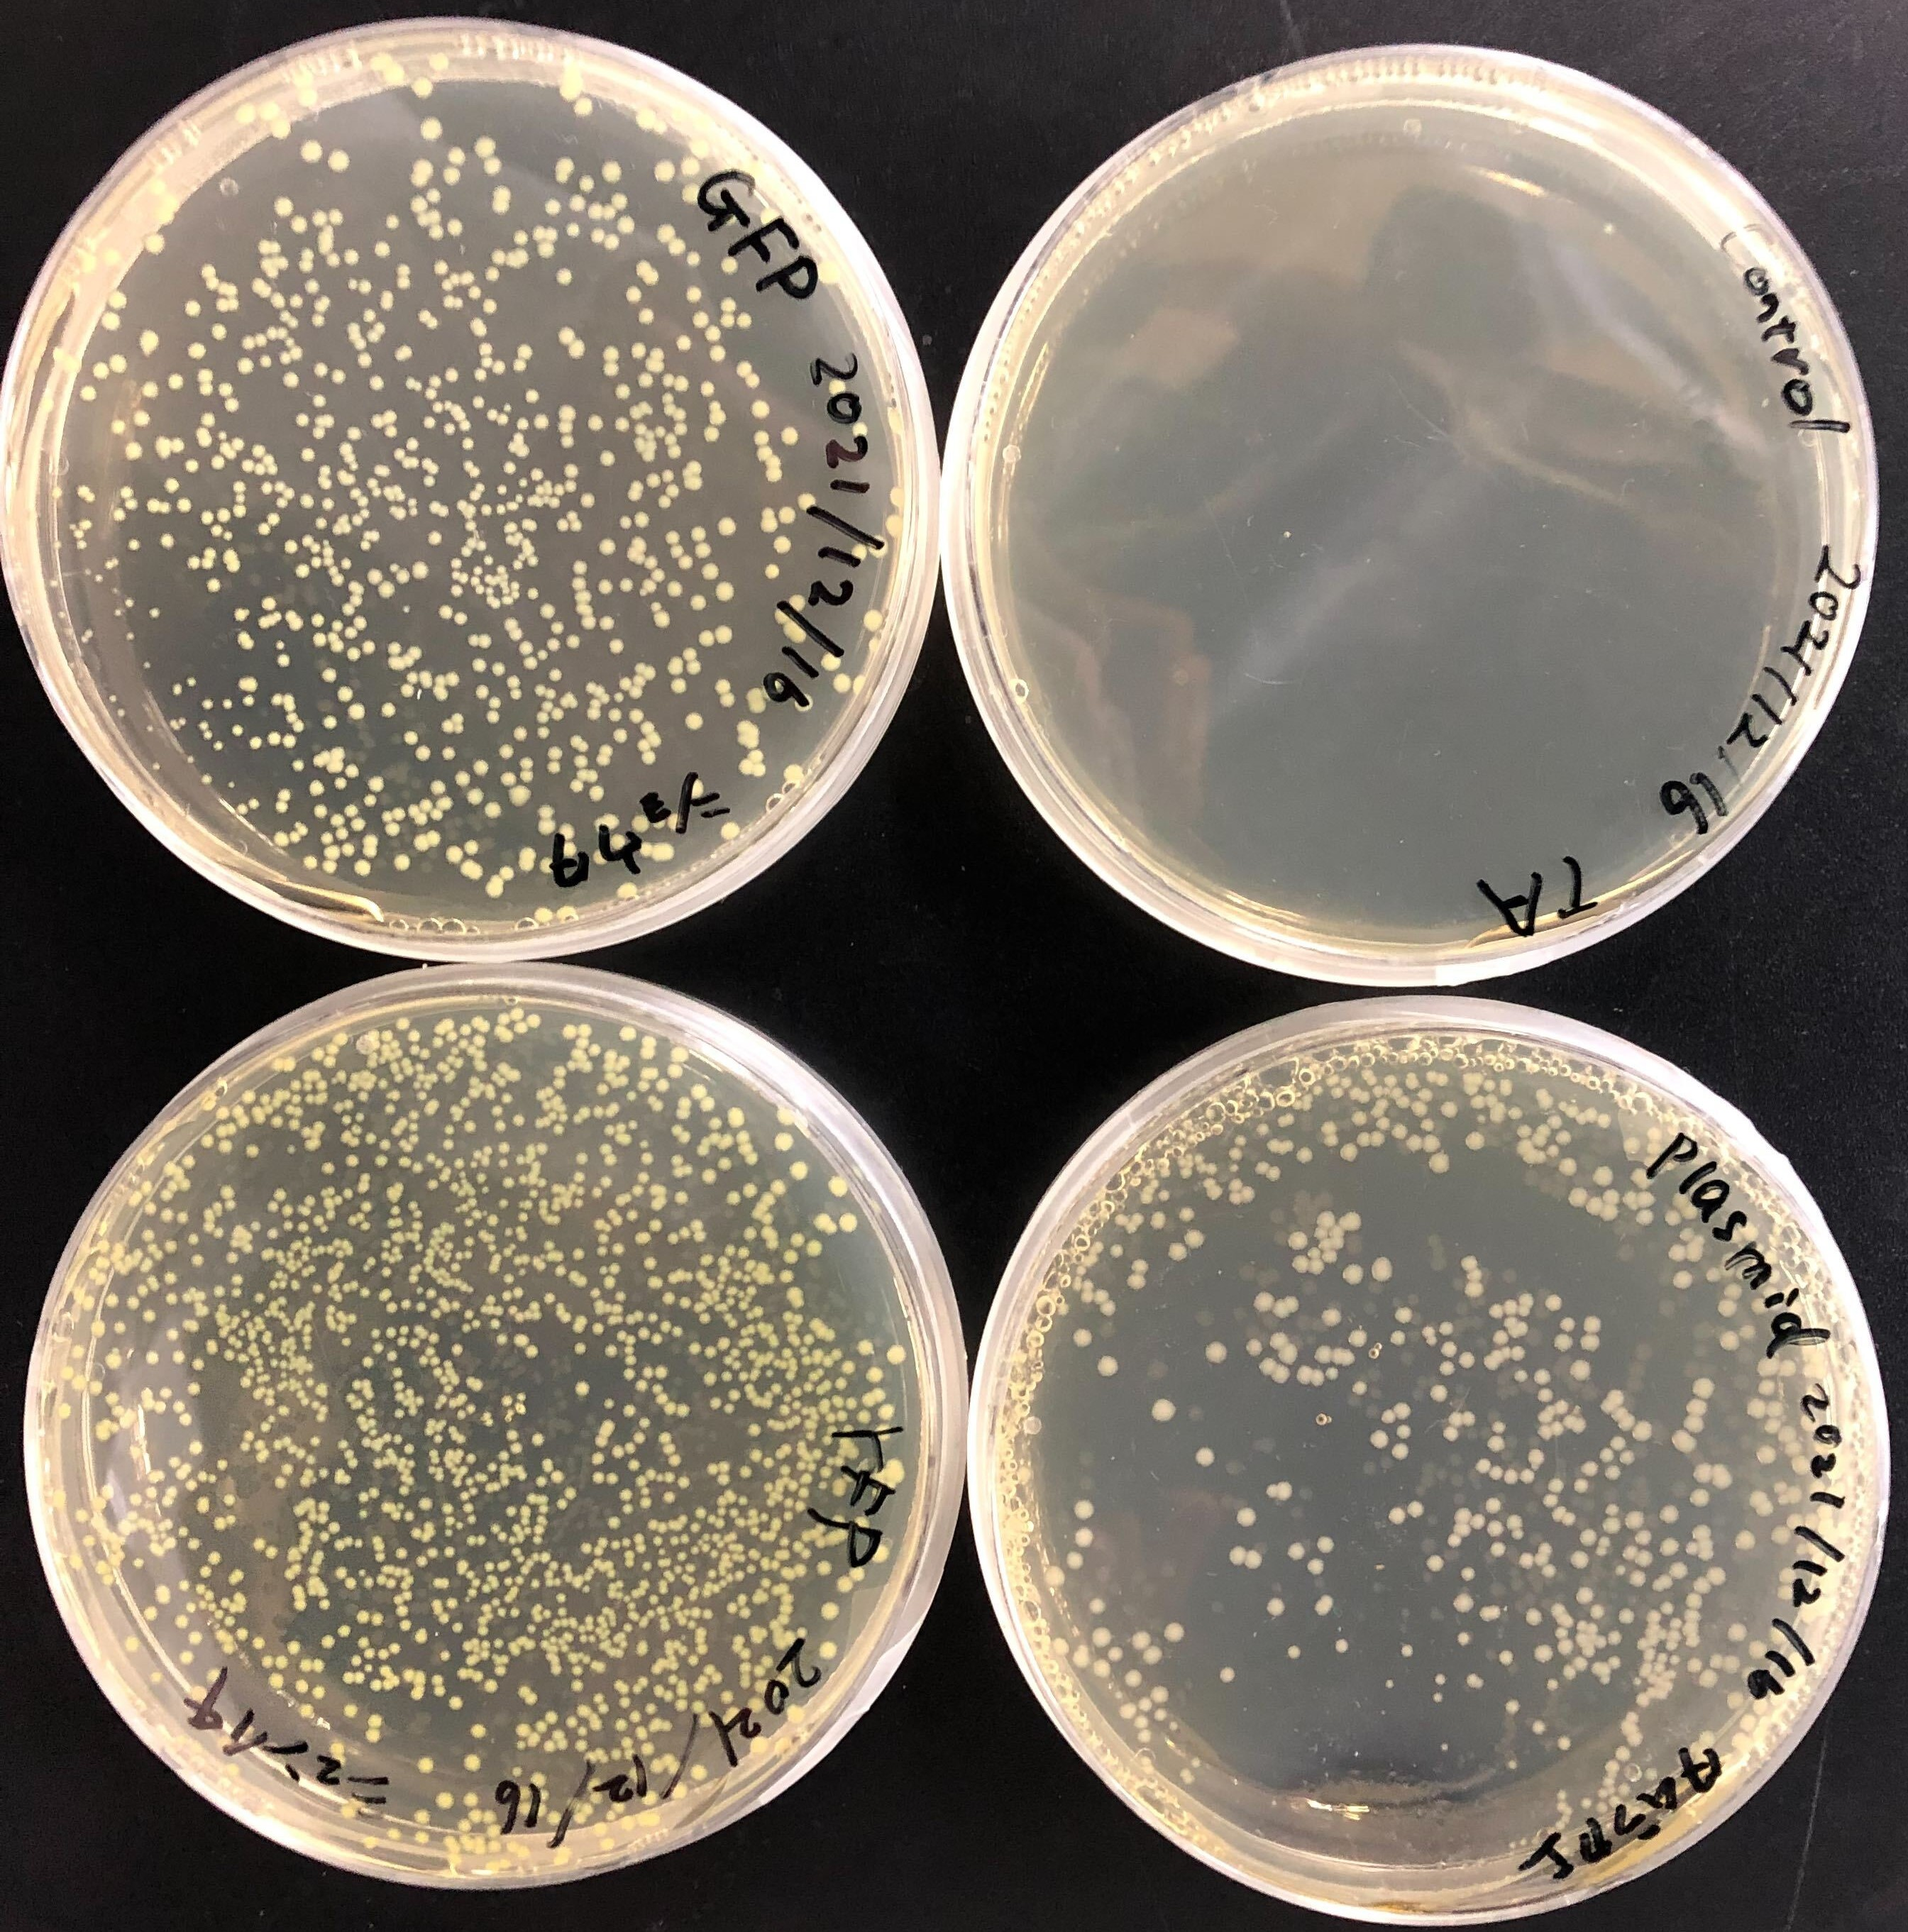
\includegraphics[width=5cm]{colonies.jpg}
    \caption{各試料のコロニーの様子.左上がGFPを入れた試料,左下がYFPを入れた試料,右上が滅菌水を入れた試料,右下がプラスミドを入れた試料.滅菌水を入れた試料以外はコロニーを形成した.}
    \label{fig:colonies}
\end{figure}

\begin{figure}[htbp]
    \centering
    \begin{subfigure}{0.3\columnwidth}
        \centering
        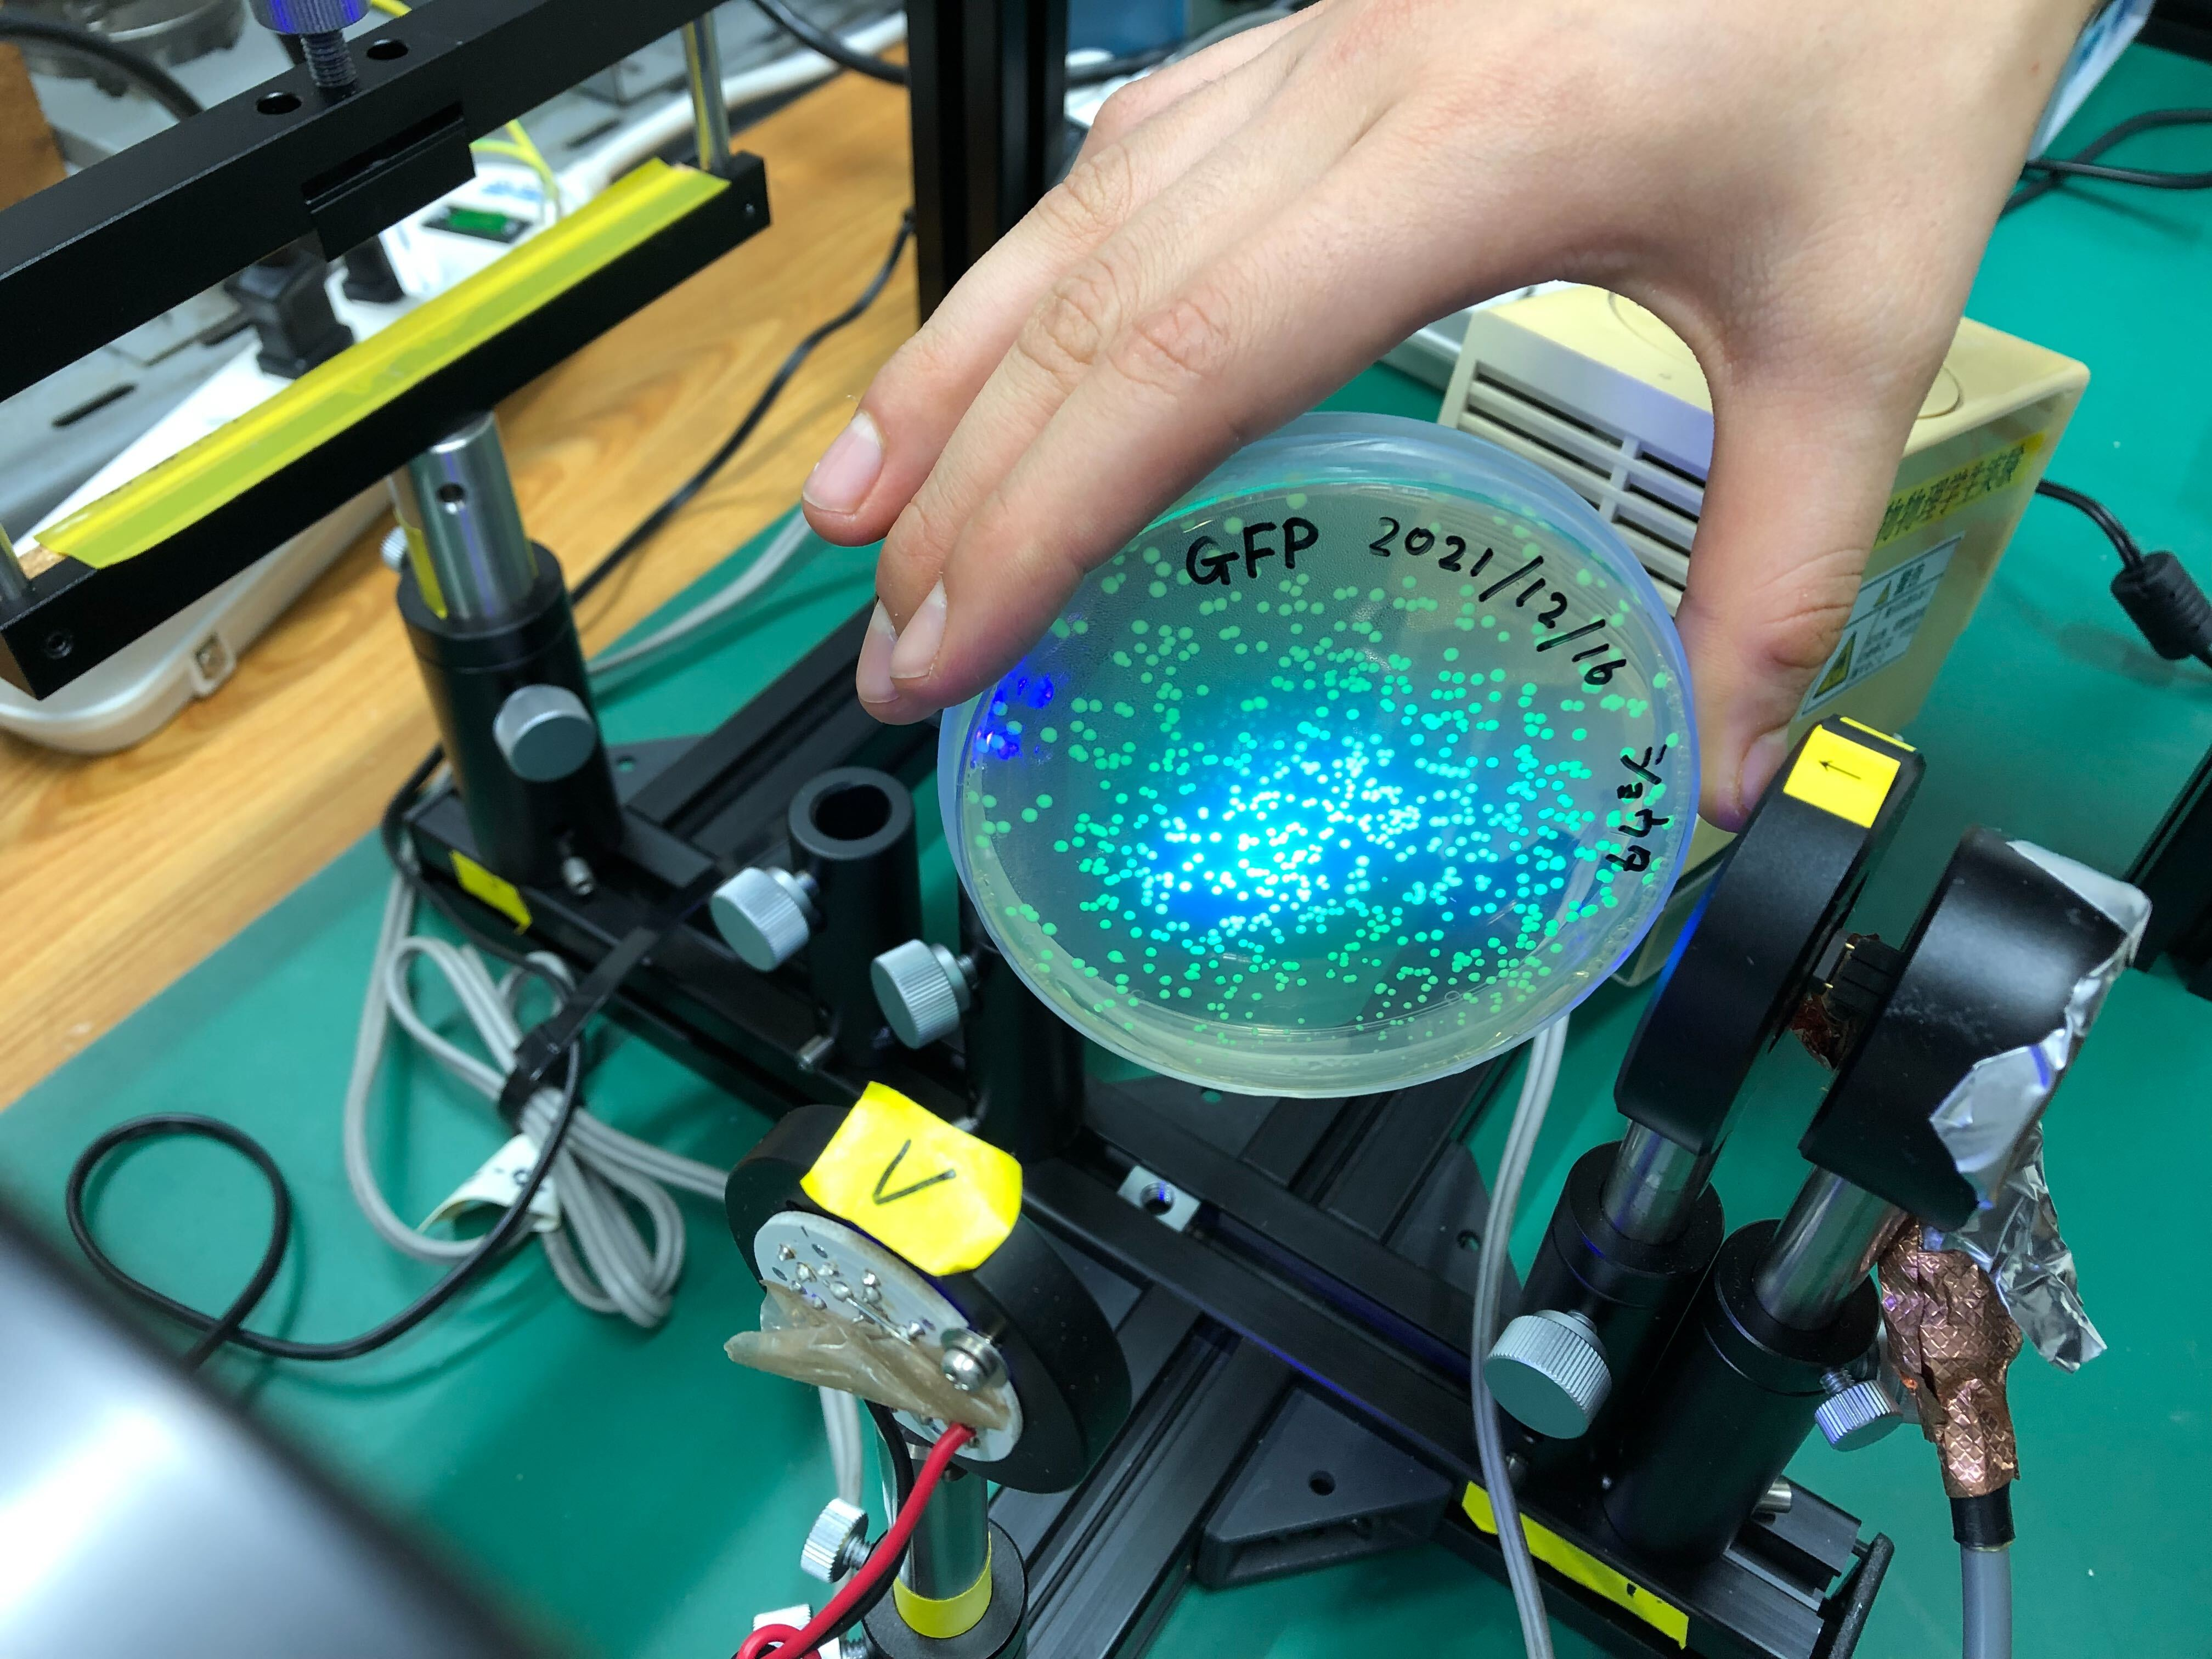
\includegraphics[width=\columnwidth]{gfp.jpg}
        \caption{GFPを入れた試料}
        \label{fig:gfp_picture}
    \end{subfigure}
    \begin{subfigure}{0.3\columnwidth}
        \centering
        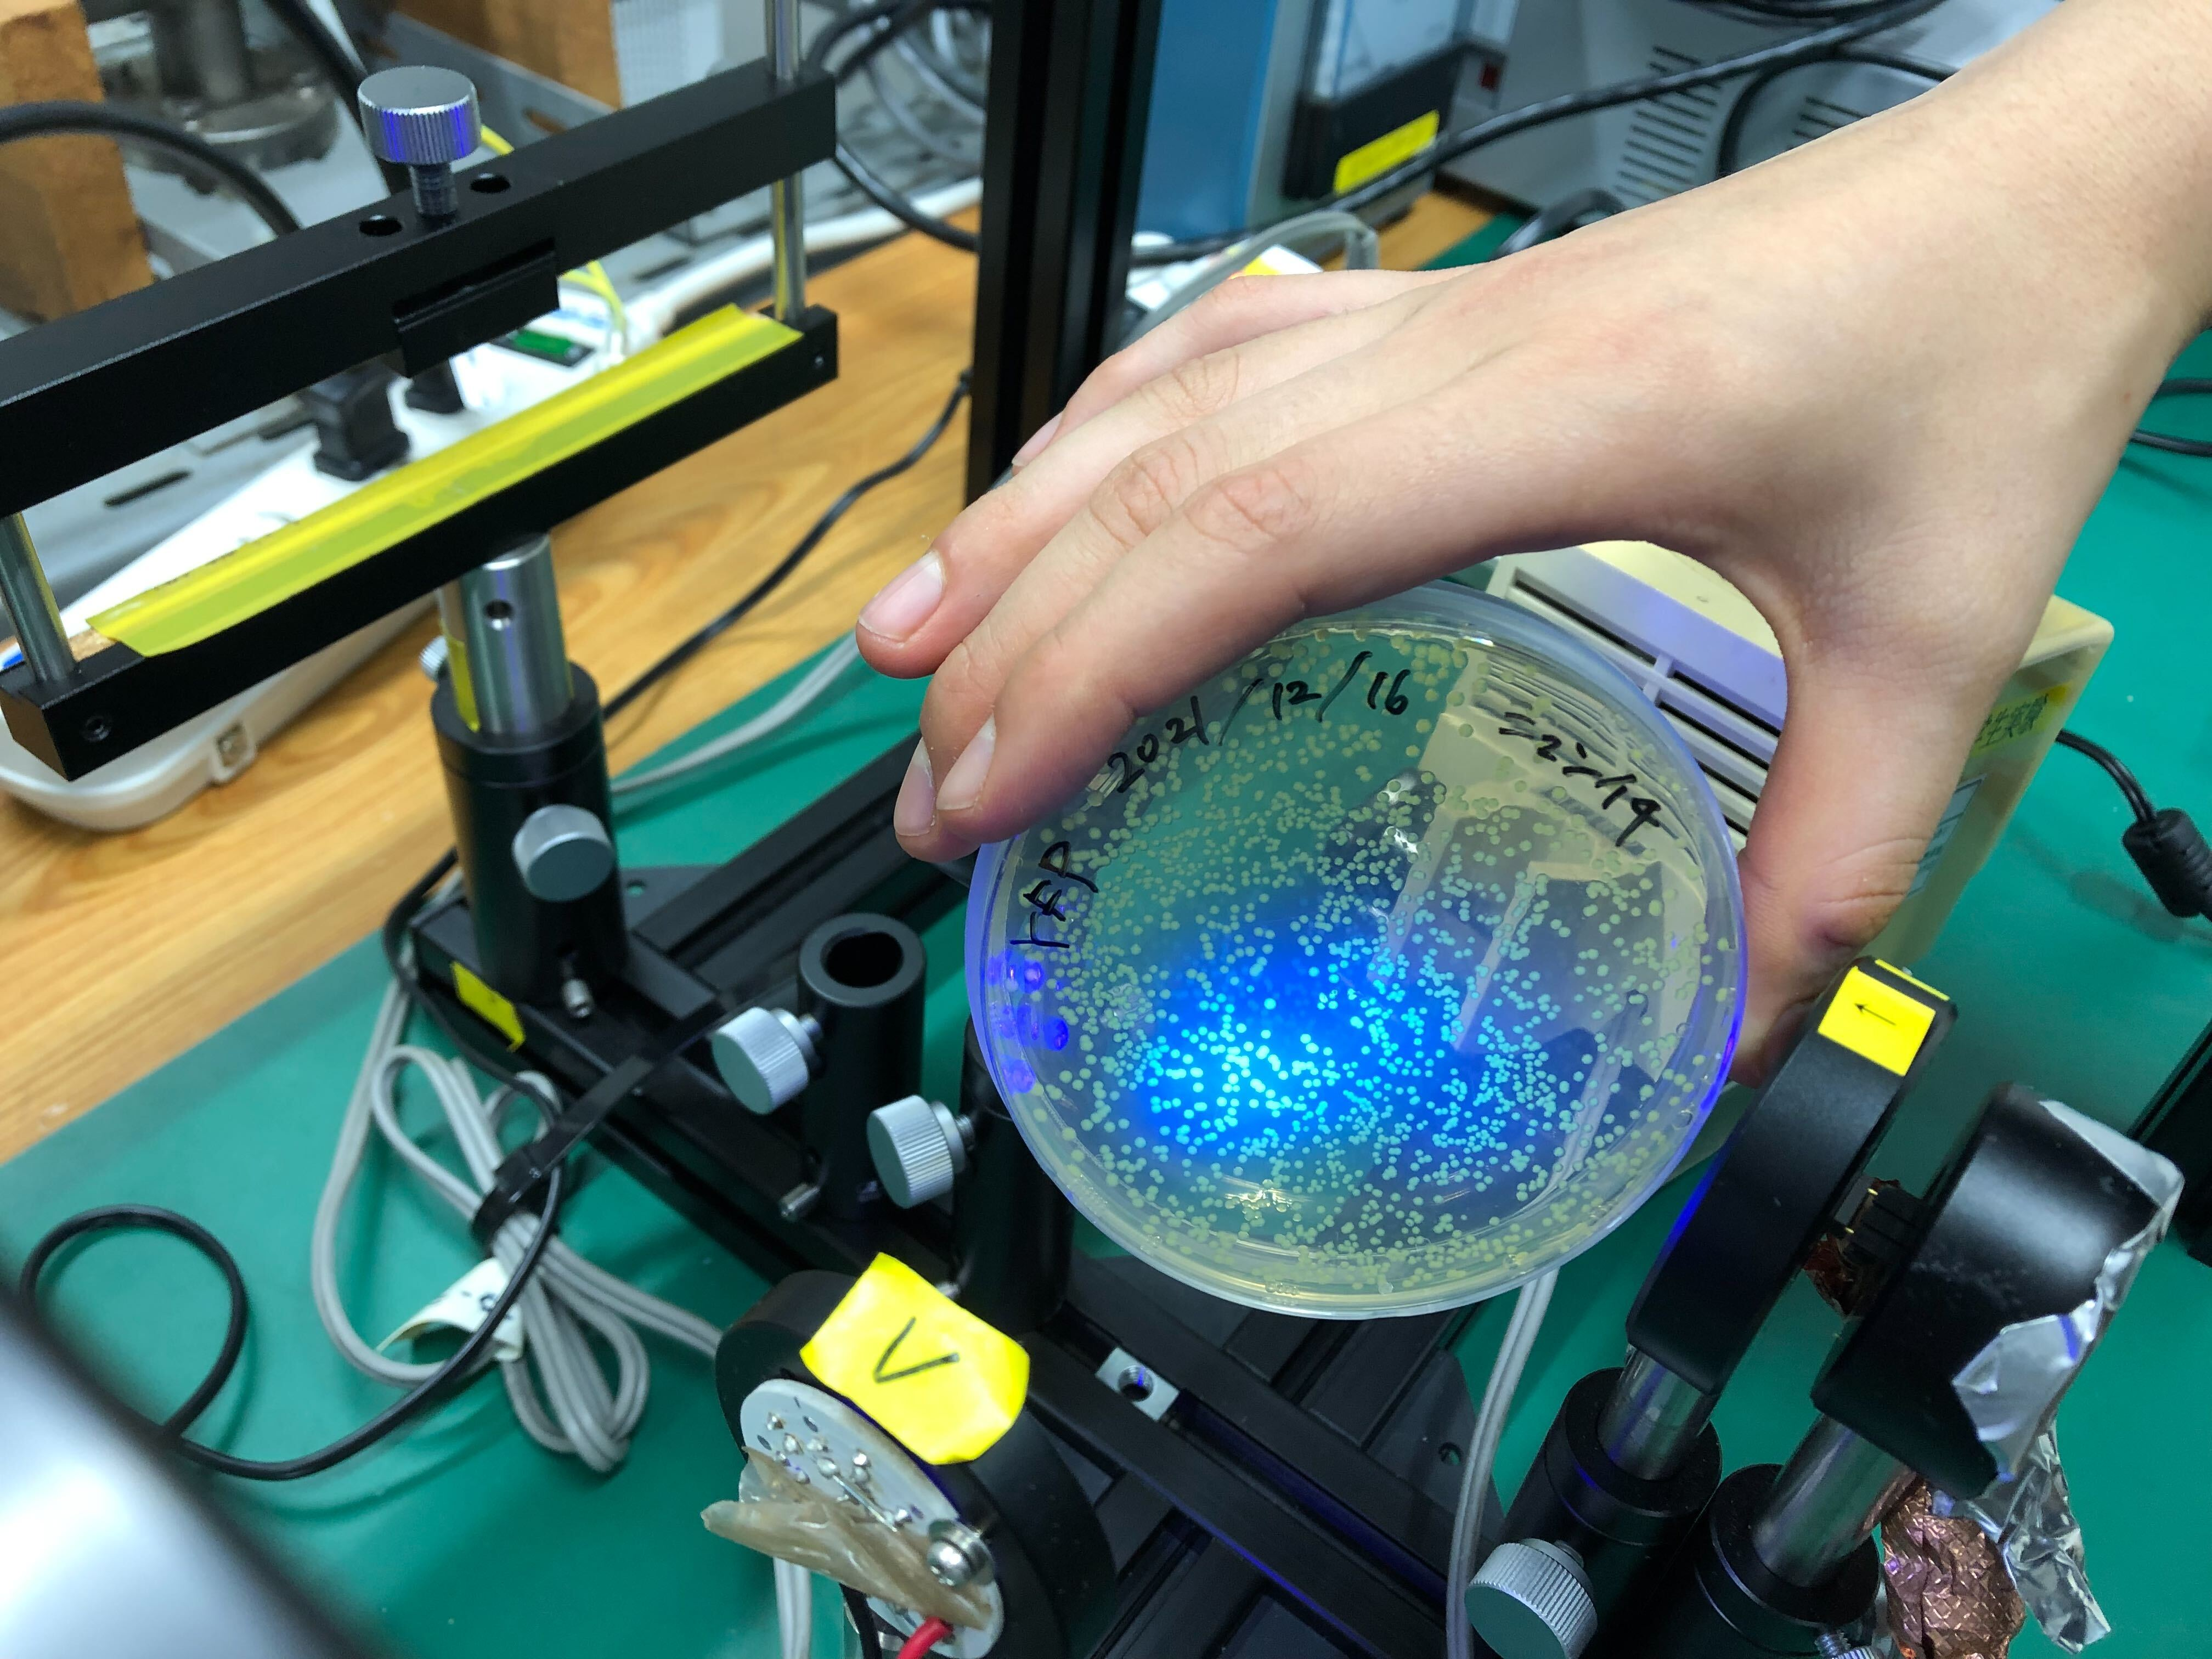
\includegraphics[width=\columnwidth]{yfp.jpg}
        \caption{YFPを入れた試料}
        \label{fig:yfp_picture}
    \end{subfigure}
    \begin{subfigure}{0.3\columnwidth}
        \centering
        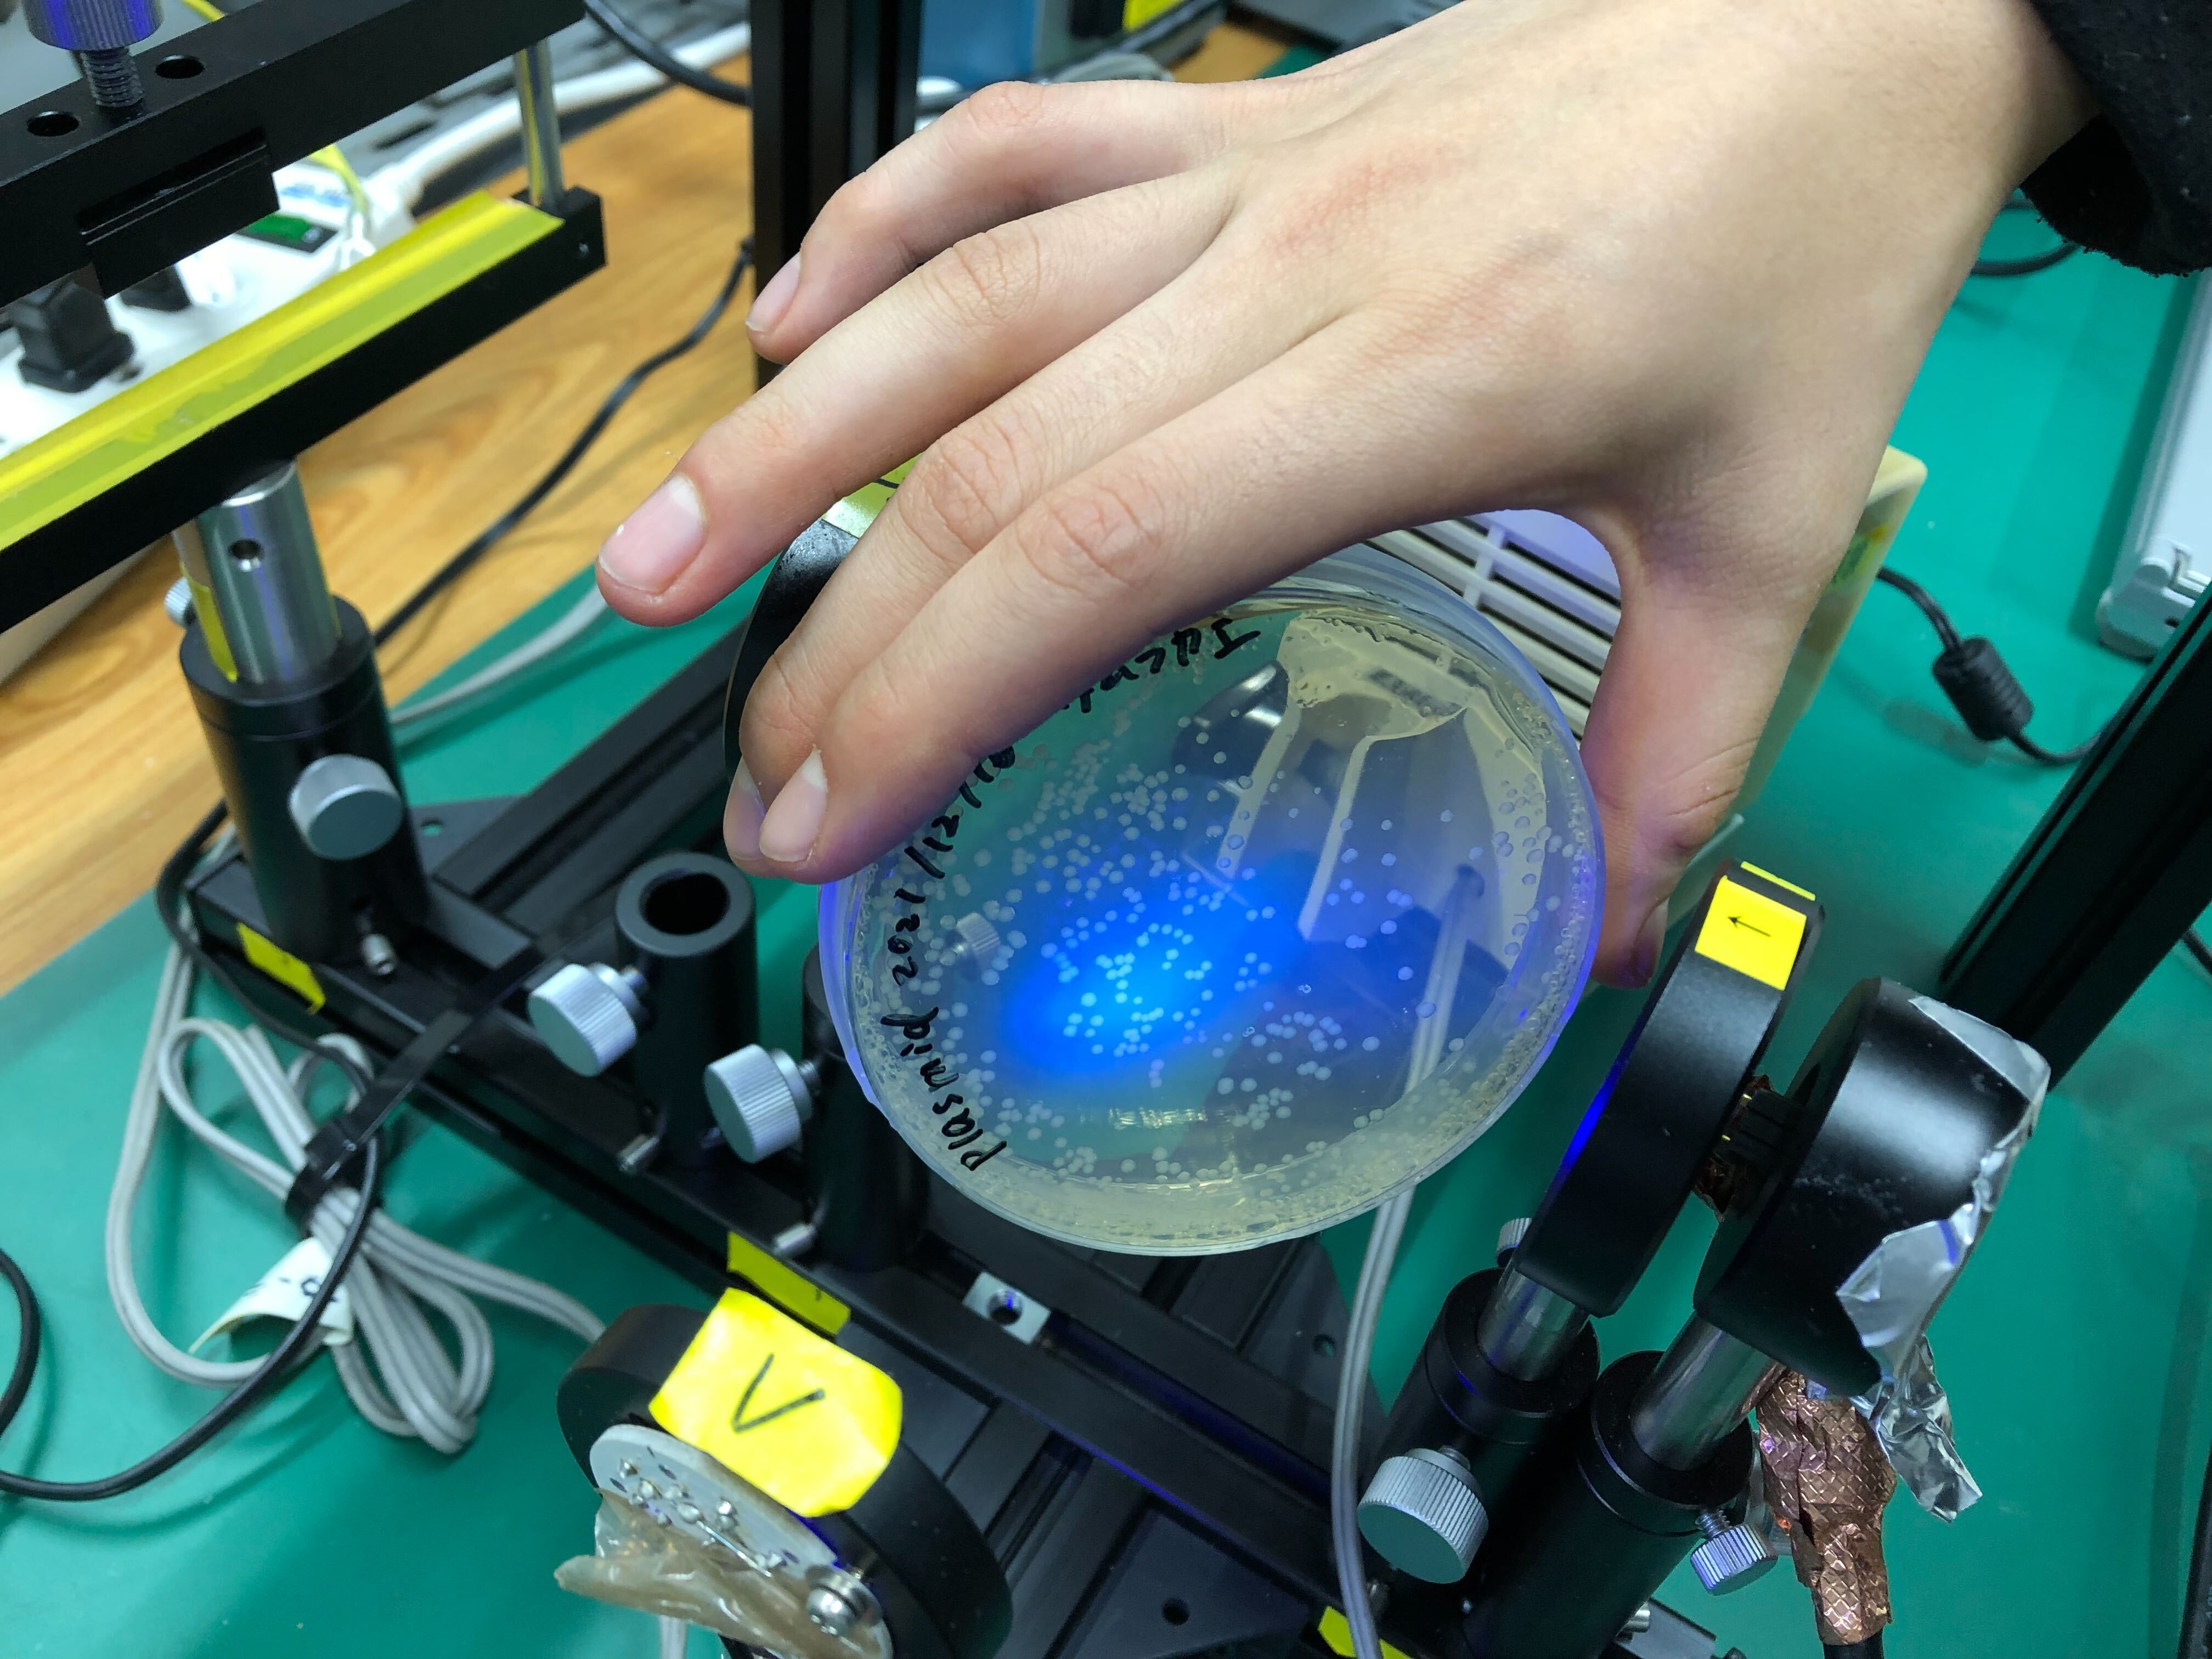
\includegraphics[width=\columnwidth]{plasmid.jpg}
        \caption{プラスミドを入れた試料}
        \label{fig:plasmid}
    \end{subfigure}    
    \caption{各試料に紫色LEDを当てたときの様子.GFPを含むプラスミドを入れた試料は強く光り,YFPを含むプラスミド入れた試料は少し光り,空のプラスミドを入れた試料は光らなかった.}
    \label{fig:purple_led}
  \end{figure}

実験の結果,滅菌水を入れた試料ではコロニーは見られず,GFP,YFPを含むプラスミドまたは空のプラスミドを入れた試料ではコロニーが多数見られた.
白色光の下では,どの試料のコロニーも白く見えた.
一方,紫色LEDの下では,GFPを入れた試料のコロニーは緑色に光って見え,YFPを入れた試料のコロニーは黄緑色に若干光って見えたが,プラスミドを入れた試料のコロニーはあまり光っていなかった.

\subsection{考察}
\subsubsection{形成されたコロニーについての考察}
コロニーが見られたのは,GFP,YFP,プラスミドの入った試料であった.
まず,この理由を考察する(課題1).
培地には抗生物質の一種であるアンピシリンが含まれていたので,コロニーを形成したのはこれに対する耐性を持った大腸菌だけであったと考える.
よって,プラスミドにはアンピシリンに対する耐性遺伝子が含まれていたと考える.
その場合,GFP,YFP,プラスミドの入った試料では,その耐性遺伝子から何らかのタンパク質がコードされ,それがアンピシリンに対する耐性をもたらしたため,コロニーを形成できたと説明できる.
一方で,滅菌水の入った試料はプラスミドを含んでいないので,アンピシリンによって死滅し,コロニーを形成できなかったと考える.

次に,コロニーに紫色LEDを当てたときの蛍光に注目して考察する(課題2).
GFPを入れた試料で観察された大腸菌は,紫色LEDに対して緑色の蛍光を発したことから,タンパク質としてのGFPが発現していたと考える.
さらに,GFPを入れた試料のコロニーはどれも蛍光を発したことから,GFPを発現させずにコロニーを形成した大腸菌は見られなかったことが分かる.
この事実は,先述したコロニーを形成できた理由の説明を裏付けている.
同様に,YFPを入れた試料で観察された大腸菌は,紫色LEDに対して黄緑色にやや光っていたことから,タンパク質としてのYFPが発現していたと考える.
蛍光がGFPほど強くなかったのは,YFPの吸収波長のピークが紫色LEDの波長よりも長波長側(緑色)にずれていたためと考える,
この試料のコロニーもすべて蛍光を発していたので,同様の考察から,先述した議論を裏付ける.

\subsubsection{タンパク質の蛍光色についての考察}

\begin{figure}[htbp]
  \centering
  \begin{subfigure}{0.3\columnwidth}
      \centering
      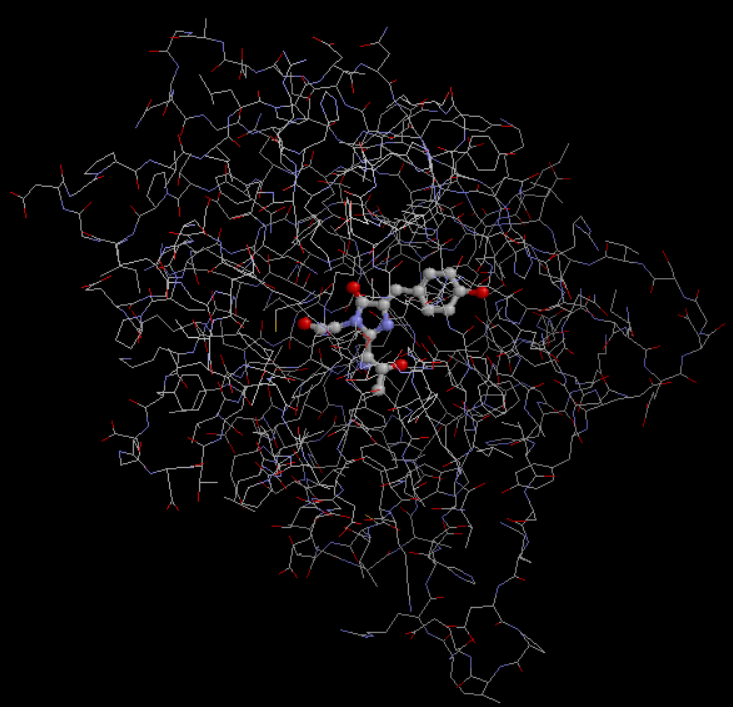
\includegraphics[width=\columnwidth]{GFP_close.png}
      \caption{GFP}
      \label{fig:GFP}
  \end{subfigure}
  \begin{subfigure}{0.3\columnwidth}
      \centering
      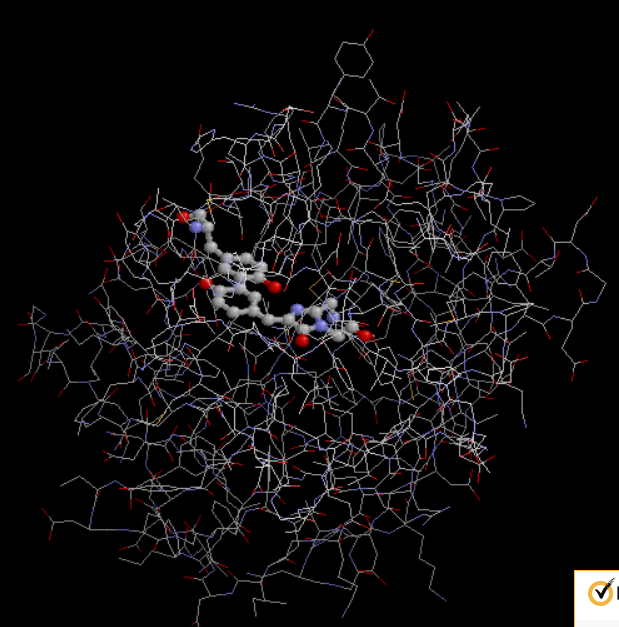
\includegraphics[width=\columnwidth]{YFP_close.png}
      \caption{YFP}
      \label{fig:YFP}
  \end{subfigure}
  \begin{subfigure}{0.3\columnwidth}
      \centering
      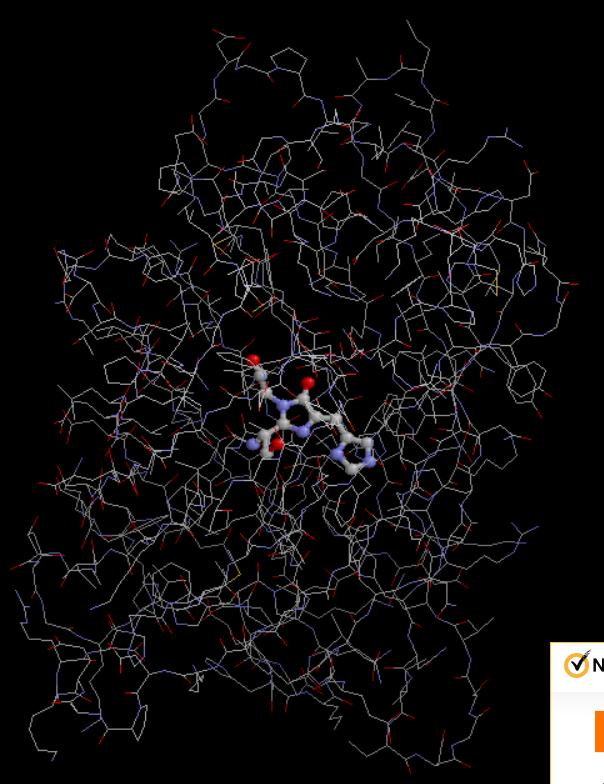
\includegraphics[width=\columnwidth]{BFP_close.png}
      \caption{BFP}
      \label{fig:BFP}
  \end{subfigure}    
  \caption{蛍光タンパク質の発色団}
  \label{fig:proteins}
\end{figure}

実験の結果,GFPは緑色,YFPは黄緑色の蛍光を発した(図\ref{fig:purple_led}).
ここでは,GFPとYFPの蛍光色を,タンパク質の発色団の構造から考察する(課題2,3).
GFPとYFPの3次元構造をそれぞれ図\ref{fig:GFP},図\ref{fig:YFP}に示す.
それぞれの図中央には,発色団を表示してある.
まず,GFPの発色団は,ベンゼン環に五員環が共役二重結合したものである.
この構造全体にわたって$\pi$電子が非局在化しており,それによって形成されるエネルギー準位のギャップに対応するエネルギーの光が吸収される.
ここでは簡単に,$\pi$電子が長さ$L$の1次元井戸型ポテンシャルに束縛されていると考える.
このときエネルギー準位は,
\begin{equation}
    E_n = \frac{h^2}{2mL^2}n^2\qquad (n=1,2,\cdots)
\end{equation}
と書ける.
ただし,$h$はプランク定数,$m$は電子の質量である.
また,吸収光の波長を$\lambda$とおくと,その光のエネルギーは光速度$c$を用いて
\begin{equation}
    \Delta E = \frac{hc}{\lambda}
\end{equation}
となる.
エネルギー準位$E_n$の中に$\Delta E$のギャップがあれば,その光は吸収される.
このようなモデル化により,$L$が長くなれば準位の間隔が狭まり,吸収される光の波長は大きくなることが推測される.
つまり,電子が広い範囲に非局在化するほど吸収波長が長くなると考える.
さらに,吸収される光の波長よりもやや長い波長の光が蛍光として観測されるので,電子の非局在化により蛍光も長波長側にシフトすると考える.

YFPの場合,GFPの203番目のアミノ酸であるスレオニンがチロシンに置き換わり,発色団のフェノール環の真上にフェノール環が接する(図\ref{fig:YFP}).
これによって$\pi$電子がさらに広範囲に非局在化し,吸収される波長が長波長側にずれると考える.
この非局在化は$\pi-\pi$スタッキングと呼ばれるようだが,詳細な原理は難しいので考察できなかった.

一方で,BFPの場合,GFPの発色団のベンゼン環が五員環に置き換わる(図\ref{fig:BFP}).
これによって$\pi$電子の動ける範囲が狭まり,吸収される波長が短波長側にずれると考える.

\subsubsection{GFPの利用}
GFPは緑色の蛍光を発するので,GFPの発現している部分を可視化できる.
さらに,GFPはタンパク質なので,今回のように遺伝子導入によって特定の細胞に発現させることができ,可視化が比較的容易である.
加えて,蛍光のために新しく何らかの物質を生体内に加える必要がない\footnote{ただし,酸素は必要である.}ため,系をほとんど乱すことなく観察できる(参考文献\cite{chemsta}).
これにより,生体内の細胞やタンパク質の動きを生きたまま観察できる.
さらに,導入する遺伝子を少し書き換えることで,YFPやBFPなど,他の色の蛍光を発するタンパク質が作られる.
このように異なる色の蛍光を発するタンパク質を合わせて使うことで,生体内の複数の部分を,それぞれ同時に可視化できる.
以上のような可視化の技術は,生物物理の研究のほか,アルツハイマーやガンといった疾患の原因究明,さらには手術の際の目印として,医療の分野にも応用されている(参考文献\cite{kahaku}).

他にもGFPには,蛍光共鳴エネルギー移動(FRET)を利用した応用がある.
これは,二つの蛍光物質の吸収波長帯が重なっているとき,一方の蛍光物質のみを励起する光を照射すると,エネルギーの移動によってもう一方の蛍光物質から蛍光が発されるという現象である.
この効果は蛍光物質間の距離が近いほど強くなる.
そのため,生体内の2つのタンパク質に異なる蛍光タンパク質を繋げれば,それらの間の距離あるいは結合強度を測定できる.

\section{二日目}
二日目は,一日目に用意したGFPおよびYFPを用いて,その吸収スペクトルおよび蛍光スペクトルを計測した.
また,GFPを酸変性させた後,塩基を加えてリフォールディングさせた.
そして,その様子を蛍光スペクトルの変化を通して観察した.

\subsection{手法}
\subsubsection{GFPおよびYFPの吸収スペクトルの測定}
まず,分光セル(石英角形吸収セル,光路長\SI{10}{\mm})にリン酸緩衝液を入れ,分光光度計(日本分光社製V-550型可視紫外分光光度計)にセットし,ベースラインを測定した.
ただし,分光光度計の設定は,測定モードをAbs,レスポンスをFast,バンド幅を\SI{2.0}{\nm},走査速度を\SI{100}{\nm\per\min},開始波長を\SI{550}{\nm},終了波長を\SI{350}{\nm},データ取り込み間隔を\SI{0.2}{\nm}とした.
次に,リン酸緩衝液のスペクトルを測定し,ベースラインが妥当であることを確認した.
そして,分光セルを洗浄した後,そこにGFP溶液を入れ,スペクトルを測定した.
同様に,YFP溶液およびリゾチーム溶液のスペクトルも測定した.

\subsubsection{YFPの蛍光強度測定}

\begin{figure}[htbp]
    \centering
    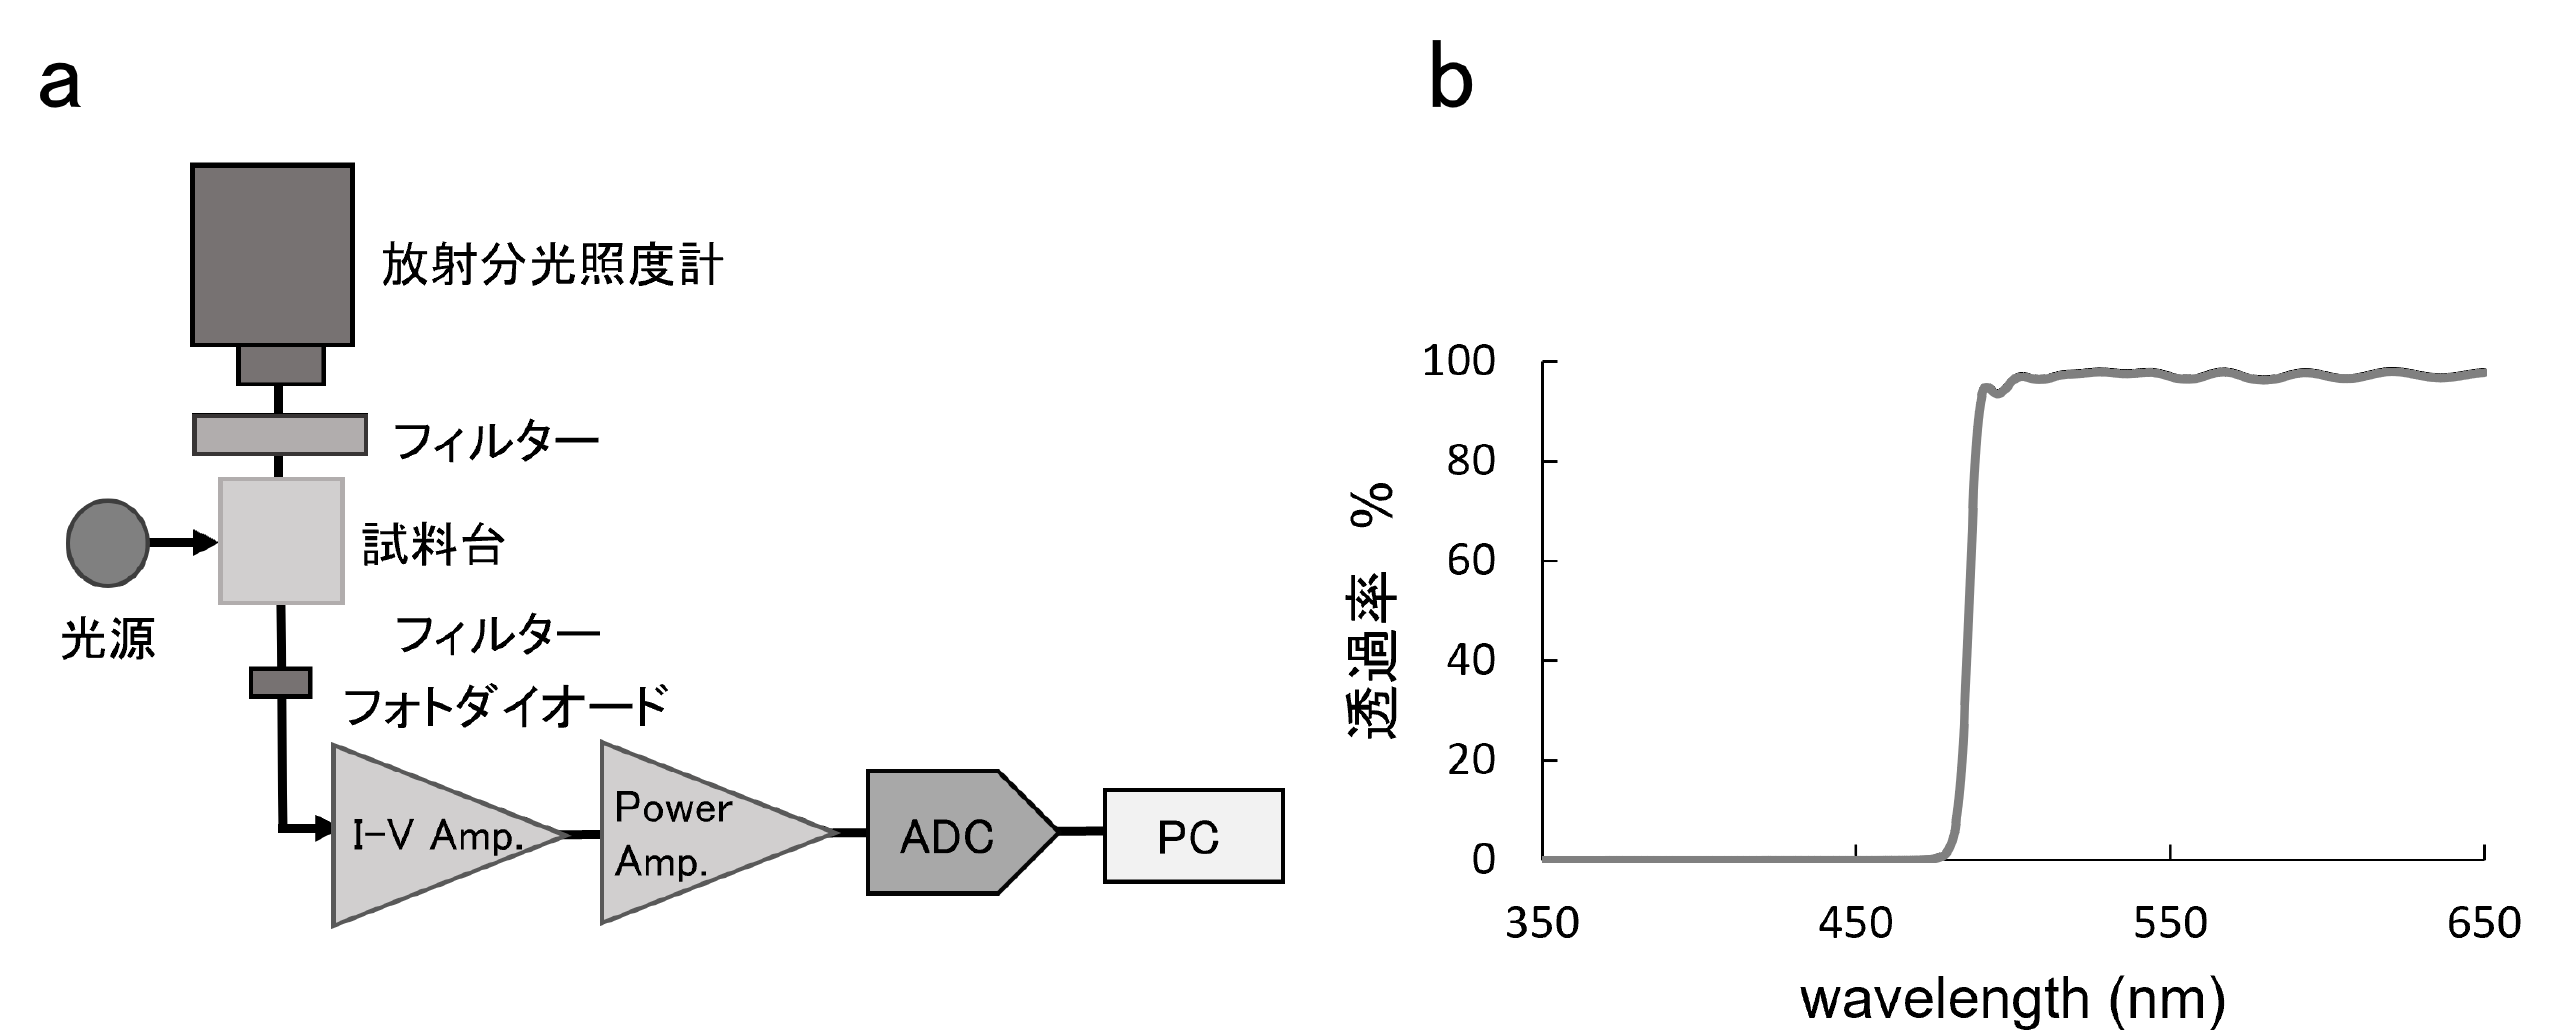
\includegraphics[width=10cm]{optical_system.png}
    \caption{(a)蛍光スペクトル測定用の光学装置の概略図.(b)光学装置に用いた短波長カットフィルターの分光特性(LVX490).ともに解説書より引用.}
    \label{fig:optical_system}
\end{figure}

まず,YFP溶液を分光セルに入れ,それを光学装置(図\ref{fig:optical_system}(a))の試料台に載せた.
次に,試料に紫色LEDを照射し,試料から出た光のスペクトルを放射分光照度計で測定した.
同様の実験をリゾチーム溶液についても行った.
最後に,励起光(紫色LED)のスペクトルも放射分光照度計で測定した.

\subsubsection{GFPの蛍光強度測定}
まず,スターラー上に撹拌子を入れたプラスチックセルを載せた.
セルにGFP溶液を\SI{2}{\milli\liter}入れ,スターラーをダイヤル6で撹拌した.
ただし,GFP溶液にプラスチックセルを入れ,スターラーを撹拌し続けた.
次に,試料に紫色LEDを照射し,放射分光照度計で天然状態のGFPの蛍光スペクトルを測定した.
その後,GFP溶液に酸(\SI{0.5}{M}\,\ce{HCl},\SI{200}{\micro\liter})を一気に加え,PC上でGFPの蛍光強度変化を測定した. 
蛍光変化が安定したところで測定を停止し,放射分光照度計で変性したGFPの蛍光スペクトルを測定した\footnote{実際には,酸を加えたときの蛍光強度変化を測定し忘れて実験を進めてしまったため,この測定だけは新しくGFP溶液を作り直して行った.}.
その後,変性したGFPの溶液に塩基(\SI{0.5}{M}\,\ce{KOH},\SI{200}{\micro\liter})を一気に加え,PC上でGFPの蛍光強度変化を測定した.
蛍光変化が安定したところで測定を停止し,放射分光照度計でリフォールディングしたGFPの蛍光スペクトルを測定した.

\subsection{結果と考察}

\subsubsection{タンパク質ごとの吸収スペクトルと蛍光スペクトル}

\begin{figure}[htbp]
    \centering
    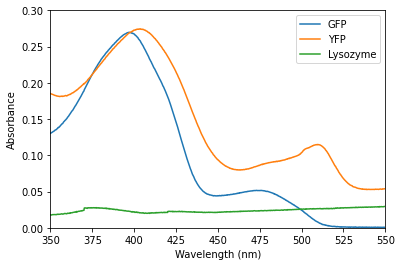
\includegraphics[width=10cm]{absorbance.png}
    \caption{GFP溶液,YFP溶液,リゾチーム溶液の吸収スペクトル}
    \label{fig:absorbance}
\end{figure}

まず,GFP溶液,YFP溶液,リゾチーム溶液の吸収スペクトルは,図\ref{fig:absorbance}のようになった.
GFP溶液の吸収スペクトルは,波長\SI{397.0}{\nm}に大きなピークが見られ,そのまわりで吸光度は下がっているものの,\SI{475}{\nm}付近にもなだらかで小さめのピークが見られた.
\SI{397.0}{\nm}のピークはGFPの発色団のフェノール基が電離していない状態に由来し,\SI{475}{\nm}付近のピークはフェノール基が電離してイオン化した状態に由来すると考える.
YFP溶液の吸収スペクトルは,波長\SI{403.8}{\nm}に大きなピークが見られ,\SI{509.6}{\nm}にも小さなピークが見られた.
この二つのピークも,GFPと同じくイオン化などによる構造の違いに由来すると考える.
一方で,リゾチーム溶液の吸収スペクトルにはそれほど強いピークは見られなかった.
ただし,全体的にゼロでない一様な吸収強度が見られたことから,ベースラインがずれてしまった可能性がある.

リゾチーム溶液に強い吸収が無いことから,GFP溶液とYFP溶液における光吸収はそれぞれタンパク質GFP,YFPによるものと考える.
この二つのスペクトルを比較すると,長波長側のピークの強さを除いて似た形状をしている.
これは一日目の実験の考察で述べた通り,GFPとYFPは発色団に同様の構造を持つためと考える.
その上で,YFPのスペクトルはGFPのスペクトルを長波長側にシフトした形をしていると読み取れる.
これもすでに述べた通り,YFPはGFPよりも広い範囲に電子が非局在化しているため,吸収波長が長くなると考えれば説明できる.

\begin{figure}[htbp]
    \centering
    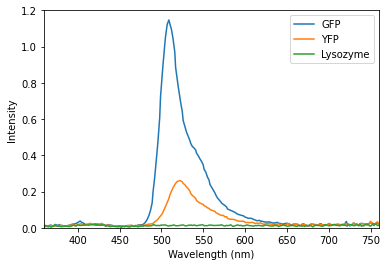
\includegraphics[width=10cm]{fluorescent.png}
    \caption{GFP溶液,YFP溶液,リゾチーム溶液の蛍光スペクトル}
    \label{fig:fluorescent}
\end{figure}

\begin{figure}[htbp]
    \centering
    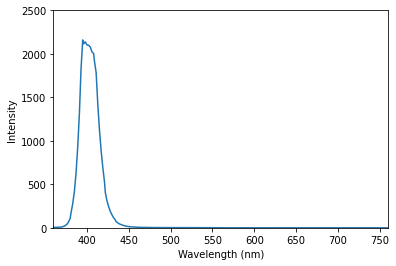
\includegraphics[width=10cm]{excitation.png}
    \caption{励起光源(紫色LED)のスペクトル.\SI{395}{\nm}で強度が最大となる.}
    \label{fig:excitation}
\end{figure}

次に,これらの溶液に紫色LEDを入射したときの蛍光スペクトルは図\ref{fig:fluorescent}のようになった.
まず,GFP溶液とYFP溶液の蛍光スペクトルは同じような形状であり,それぞれ波長\SI{509}{\nm},\SI{522}{\nm}にピークが見られた.
一方で,リゾチーム溶液にはピークは見られなかった.
また,励起光(紫色LED)のスペクトルは図\ref{fig:excitation}のようになり,波長\SI{395}{\nm}に吸光ピークが見られた.
GFPの蛍光ピークがYFPのそれと比べて大きいのは,この励起光がGFPの蛍光のために吸収される波長領域に集中しており,YFPの蛍光のための吸収波長の領域からは少しずれているためと考える.
具体的には,YFPの蛍光はGFPの蛍光よりも長波長なので,励起波長もYFPの方が長い.
そのため,YFPの励起波長は紫色LEDのスペクトルのピークよりも長波長側にずれていると考える.

\subsubsection{GFPの天然状態,変性状態,リフォールディング状態における蛍光スペクトル}

\begin{figure}[htbp]
    \centering
    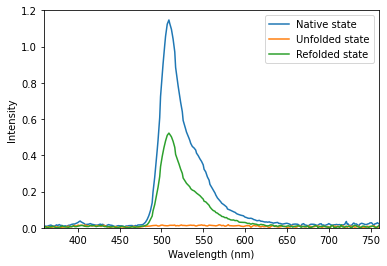
\includegraphics[width=10cm]{fluore_protein.png}
    \caption{GFPの天然状態、変性状態,リフォールディング状態における蛍光スペクトル}
    \label{fig:fluore_protein}
\end{figure}

GFPの天然状態と,そこに酸を加えた後の変性状態,およびそこにさらに塩基を加えた後のリフォールディング状態における蛍光スペクトルは,図\ref{fig:fluore_protein}のようになった.
変性状態ではピークは見られず,天然状態とリフォールディング状態はともに波長\SI{509}{\nm}にピークが見られた.
蛍光スペクトルのピークの位置が等しいことから,リフォールディングによって再び同じ構造のGFPが復元したと考える.
また,リフォールディング状態は天然状態と比べて蛍光強度が半分程度に減っていた.
これは,リフォールディング状態での溶液中のGFP濃度が,もとのGFP濃度よりも低いことを意味する.
そこでまず,体積の増加による寄与を考える.
今回の実験では,リフォールディング後のGFP溶液の体積は,酸や塩基を加えた分,最初のGFP溶液の体積より大きい.
しかし,もとの体積\SI{2}{\milli\liter}が\SI{2.4}{\milli\liter}に増加しただけ(増分は20\%)なので,蛍光強度が半分以下になることは説明できない.
よって,この結果は,すべてのGFPが復元したわけではないことを意味する.
たとえば,酸によって何らかの結合が切断されてしまったGFPはリフォールディングされないと考える.

\subsubsection{GFPの変性過程}

\begin{figure}[htbp]
    \centering
    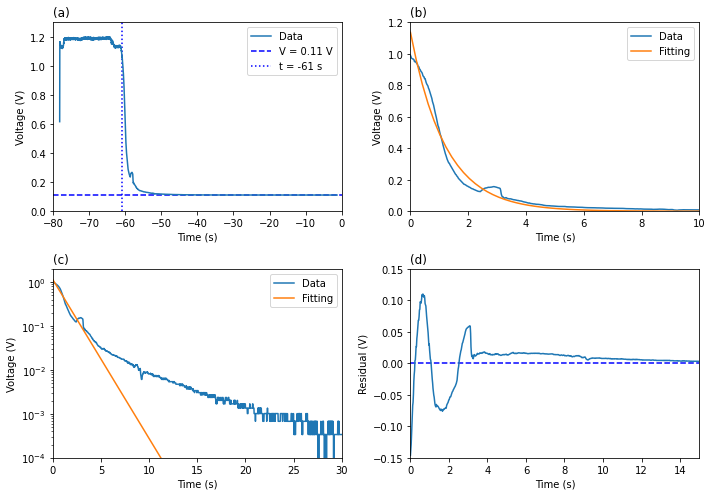
\includegraphics[width=14cm]{unfolding.png}
    \caption{(a)変性過程の電圧値の推移.グラフをもとに,立ち下がりの時刻(\SI{-61}{\second})と平衡電圧(\SI{0.11}{\volt})を記録した.以降では,立ち下がりの時刻を0,平衡電圧を0とする時刻および電圧を採用する.(b)立ち下がり以降の電圧の曲線をsingle exponentialでフィットした結果.縦軸を対数にとると,(c)が得られた.(d)フィッティングの残差.}
    \label{fig:unfolding}
\end{figure}

最後に,GFP溶液に酸を加えたときの変性過程,およびそこに塩基を加えたときのリフォールディング過程における蛍光強度の推移について考察する.

まず,変性過程の蛍光強度の推移は図\ref{fig:unfolding}(a)のようになった.
これより,蛍光強度の立ち下がりの時刻は\SI{-61}{\second},変性後の平衡電圧は\SI{0.11}{\volt}と読み取れる.
ここで,時刻$t$および電圧$V$を,この立ち下がり時刻および平衡電圧を0とするようにそれぞれ定義し直した.
以降では,新しく定義したこの時刻と電圧を用いる.
次に,立ち下がり以降の蛍光強度の曲線を
\begin{equation}
    V = A\exp(-\frac{t}{\tau})
\end{equation}
でフィッティングしたところ,パラメータは
\begin{equation}
    A = \SI[separate-uncertainty]{1.137 \pm 0.004}{\volt}, \qquad
    \tau = \SI[separate-uncertainty]{1.200 \pm 0.006}{\second}
\end{equation}
と求まった.
実験結果はフィッティング曲線に沿っているものの,時刻の小さい領域でずれが見られた(図\ref{fig:unfolding}(b)).
とくに酸を入れた直後の蛍光強度の変化は,フィッティング曲線と比較して非常に緩やかであった.
時刻\SI{3}{\second}付近にも山が見られるが,これはノイズと考える.
また,図\ref{fig:unfolding}(b)の縦軸を対数にとり,より時刻の大きい部分も含めて図示すると,図\ref{fig:unfolding}(c)のようになった.
これより,時刻$t > \SI{5}{\second}$ではフィッティングで求めた時定数は実験結果と乖離していることが読み取れる.
このことから,実験結果はsingle exponentialでは説明できないと考える.
フィッティングの残差を示すと図\ref{fig:unfolding}(d)のようになり,残差は時刻$t < \SI{3.5}{\second}$で大きく振動しており,その後は緩やかに減衰していることが分かる.
残差についてのこれ以上の考察は,リフォールディング過程の結果と比較して行う.

\begin{figure}[htbp]
    \centering
    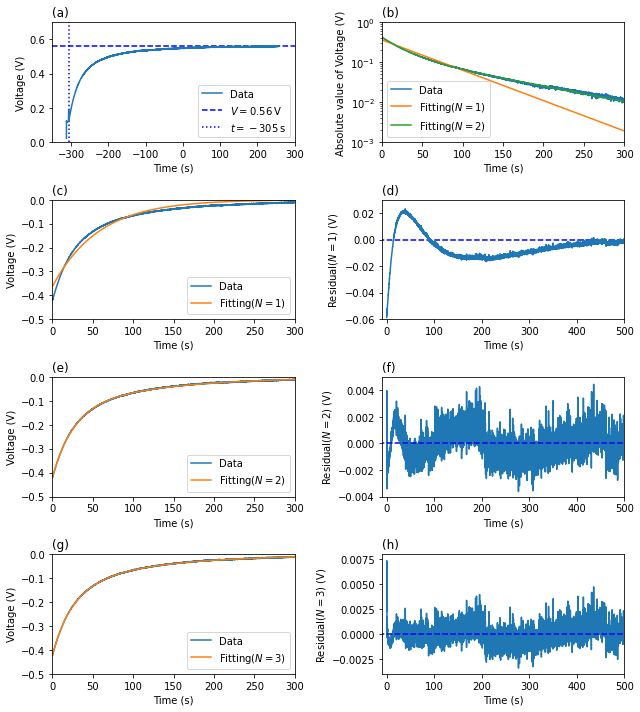
\includegraphics[width=14cm]{refolding.png}
    \caption{(a)リフォールディング過程の電圧値の推移。グラフをもとに,立ち上がりの時刻(\SI{-300}{\second})と平衡電圧\SI{0.56}{\volt}を記録し,以降ではこれらを0とする時刻と電圧を定義し直して用いる.(b)実験結果とフィッティング結果の比較.縦軸は電圧値の絶対値にとった.ここで,フィッティングは複数のexponentialの線形結合で行った.その結果,2項で十分精度良く近似できた.single exponentialによるフィットは(c),残差は(d)のようになった.2項のexponentialによるフィットは(e),残差は(f)のようになった.また,3項のexponentialによるフィットは(g),残差は(h)のようになった.}
    \label{fig:refolding}
\end{figure}

\subsubsection{GFPのリフォールディング過程}

次に,リフォールディング過程の蛍光強度の推移は図\ref{fig:refolding}(a)のようになった.
これより,蛍光強度の立ち上がりの時刻は\SI{-300}{\second},リフォールディング後の平衡電圧は\SI{0.56}{\volt}と読み取れる.
先ほどと同様,以降ではこれらを0とする時刻$t$と電圧$V$を定義し直して用いる\footnote{変性過程のときと異なり,$V$は常に負になる.}.
次に,実験結果を
\begin{equation}
    V = -\sum_{i=1}^{N} A_i \exp(-\frac{t}{\tau_i})
\end{equation}
の形でフィッティングした.
その結果,パラメータは$N=1$の場合
\begin{equation}
    A_1 = \SI[separate-uncertainty]{0.3626\pm 0.0008}{\volt}, \qquad \tau_1 = \SI[separate-uncertainty]{57.05\pm 0.17}{\second}
\end{equation}
となり,$N=2$の場合
\begin{align}
    A_1 = \SI[separate-uncertainty]{0.1492\pm 0.0003}{\volt},\qquad \tau_1 = \SI[separate-uncertainty]{112.44\pm 0.15}{\second}\\
    A_2 = \SI[separate-uncertainty]{0.2707\pm 0.0003}{\volt},\qquad \tau_2 = \SI[separate-uncertainty]{24.92\pm 0.04}{\second}
\end{align}
となり,$N=3$の場合
\begin{align}
    A_1 = \SI[separate-uncertainty]{0.1332\pm 0.0008}{\volt}, \qquad \tau_1 = \SI[separate-uncertainty]{118.5\pm 0.3}{\second}\\
    A_2 = \SI[separate-uncertainty]{0.208\pm 0.007}{\volt}, \qquad \tau_2 = \SI[separate-uncertainty]{31.5\pm 0.5}{\second}\\
    A_3 = \SI[separate-uncertainty]{0.083\pm 0.007}{\volt}, \qquad \tau_3 = \SI[separate-uncertainty]{15.4\pm 0.5}{\second}
\end{align}
となった.
ここで,$N=1$と$N=2$のフィッティングを実験結果とともに図示すると図\ref{fig:refolding}(b)のようになった.
ただし,縦軸は電圧の絶対値の対数とした.
これより,$N=1$に比べて$N=2$は実験結果にフィットすることが分かる.
$N=3$の場合はほとんど$N=2$と重なっていたので,この図には記載しなかった.

$N=1$のフィッティングは図\ref{fig:refolding}(c)のように,実験結果とおおよそ合っているものの,時間変化の仕方が過度に緩やかである.
これにより,フィッティングの残差(図\ref{fig:refolding}(d))は系統的に0から外れている.
一方で,$N=2$のフィッティングは図\ref{fig:refolding}(e)のように,実験結果とほとんど違いが見られない.
その残差(図\ref{fig:refolding}(f))を確認すると,残差の振れ幅が$N=1$のときと比べて10分の1程度に抑えられていることが分かる.
ただし,残差はやや波打っており,とくに塩基を入れた直後の時刻($t=\SI{0.25}{\second}$付近)では急激に変化していることが分かる.
最後に,$N=3$のフィッティングは図\ref{fig:refolding}(g)のように,実験結果とほぼ重なっている.
その残差(図\ref{fig:refolding}(h))を確認すると,$N=2$のときに見られた,$t=\SI{50}{\second}$付近のフィッティングのずれがやや改善している.
しかし,塩基を入れた直後($t=\SI{0.25}{\second}$付近)のフィッティングのずれは悪化している.

ここで,$N=1,2,3$のうちフィッティングとして最良なものは$N=2$と考える.
というのは,フィッティングの結果得られたパラメータの誤差は$N=2$のとき最小だからである.
ただし,$N=2,3$のフィッティングの残差にはいずれも周期の大きな波が見られるので,$N=4$以降までとればさらに良いフィッティングが得られる可能性はある\footnote{実際に試したが,初期値が不適だったためかパラメータの誤差が大幅に増加してしまったため,ここには載せられなかった.}.

\begin{figure}[htbp]
    \centering
    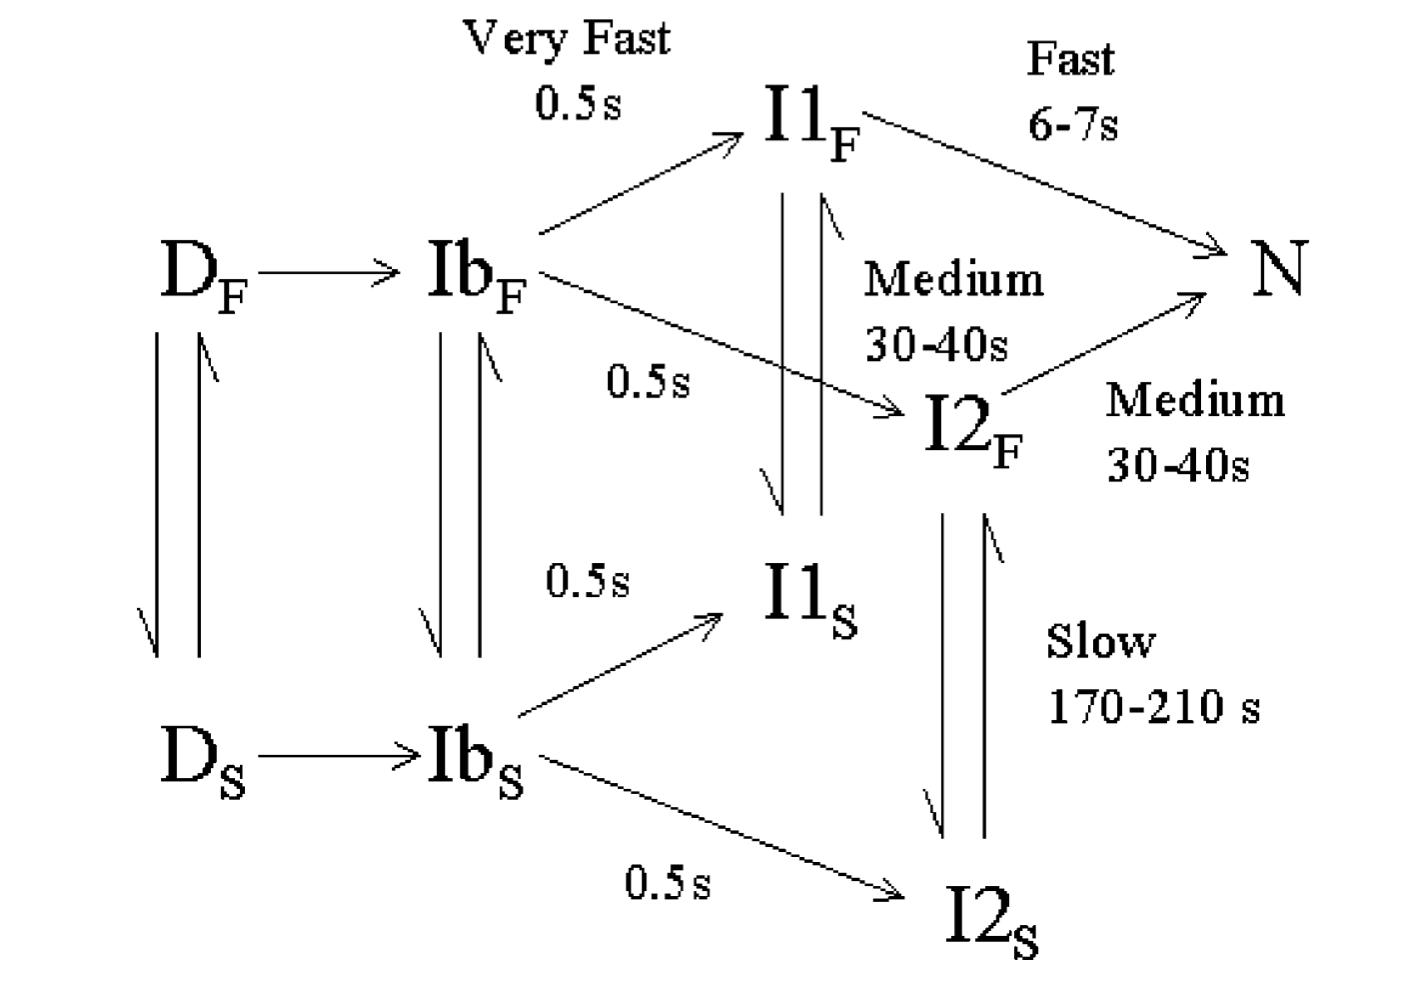
\includegraphics[width=10cm]{ref_pathway.png}
    \caption{GFPのリフォールディング過程の反応経路の概略図.D$_\mathrm{S}$とD$_\mathrm{F}$は酸変性した状態を意味し,Nは自然状態を意味する.(出典:Enoki et al.(2004)\cite{refolding})}
    \label{fig:ref_path}
\end{figure}

$N=2$のフィッティングによれば,GFPのリフォールディングの時定数は,\SI{112.44}{\second}と\SI{24.92}{\second}の二通りある.
これは,GFPのリフォールディングが複数の異なる反応経路によって行われるためと考える.
この反応経路について,Enoki, Saeki, Maki, \& Kuwajima(2004)の論文\cite{refolding}では,図\ref{fig:ref_path}のようなスキームが紹介されていた.
これをもとに考えると,今回の実験で得られた時定数\SI{112.44}{\second}は中間体I2$_\mathrm{S}$から中間体I2$_\mathrm{F}$への反応に由来し,\SI{24.92}{\second}は中間体I1$_\mathrm{S}$から中間体I1$_\mathrm{F}$への反応または中間体I2$_\mathrm{F}$から自然状態Nへの反応に由来すると考える.
また,このスキームから,今回$N=2$で導いた時定数のほかにも時定数が隠れていると考える.

\subsubsection{GFPの変性過程とリフォールディング過程の比較}

最後に,変性過程とリフォールディング過程を比較して,変性過程のsingle exponentialによるフィッティングの精度があまり良くない理由を考察する.
まず,変性過程のフィッティングから外れているのは,酸を入れた直後に電圧が緩やかに変化するところである.
これは,フラスコに酸が入って徐々に拡散したことによると考える.
実際,リフォールディング過程においても,塩基を入れた直後はフィッティングのずれが比較的大きかった.
このことから,変性過程とリフォールディング過程に共通する物質の拡散過程が,変性過程の実験結果とフィッティングのずれの原因と考える.

これをもとに考えると,今回の実験では,酸が拡散する過程とGFPの変性の時定数が近かったことで,酸が拡散しきる前に変性が始まったため,変性過程の蛍光強度の振る舞いはsingle exponentialから外れたと考える.
一方で,塩基が拡散する過程に比べてGFPのリフォールディングの時定数(数十秒程度)は十分大きい.
そのため,塩基が拡散しきってからリフォールディングが始まり,リフォールディングの時定数を持ったexponentialの項によって精度良くフィッティングできたと考える.

\section{三日目}
\subsection{手法}
\subsubsection{水銀ランプと励起フィルターの透過光のスペクトル測定}
まず,放射分光照度計を用いて,水銀ランプおよび励起フィルターを透過した光のスペクトルを測定した.
励起フィルターの透過光は,蛍光ミラーユニットとしてU-MWIG3(テトラメチルローダミン用)とU-MGFPHQ(GFP用)の二つを使用し,それぞれの場合について測定した.
これらの蛍光ミラーユニットは,後の実験では蛍光顕微鏡内に\ref{fig:scope}のように配置して用いた.
これにより,光源のうち特定の波長範囲の光を励起光としてサンプルに照射でき,かつサンプルから出た光のうち蛍光の波長範囲のみを選択的に撮影できる.

\begin{figure}[htbp]
    \centering
    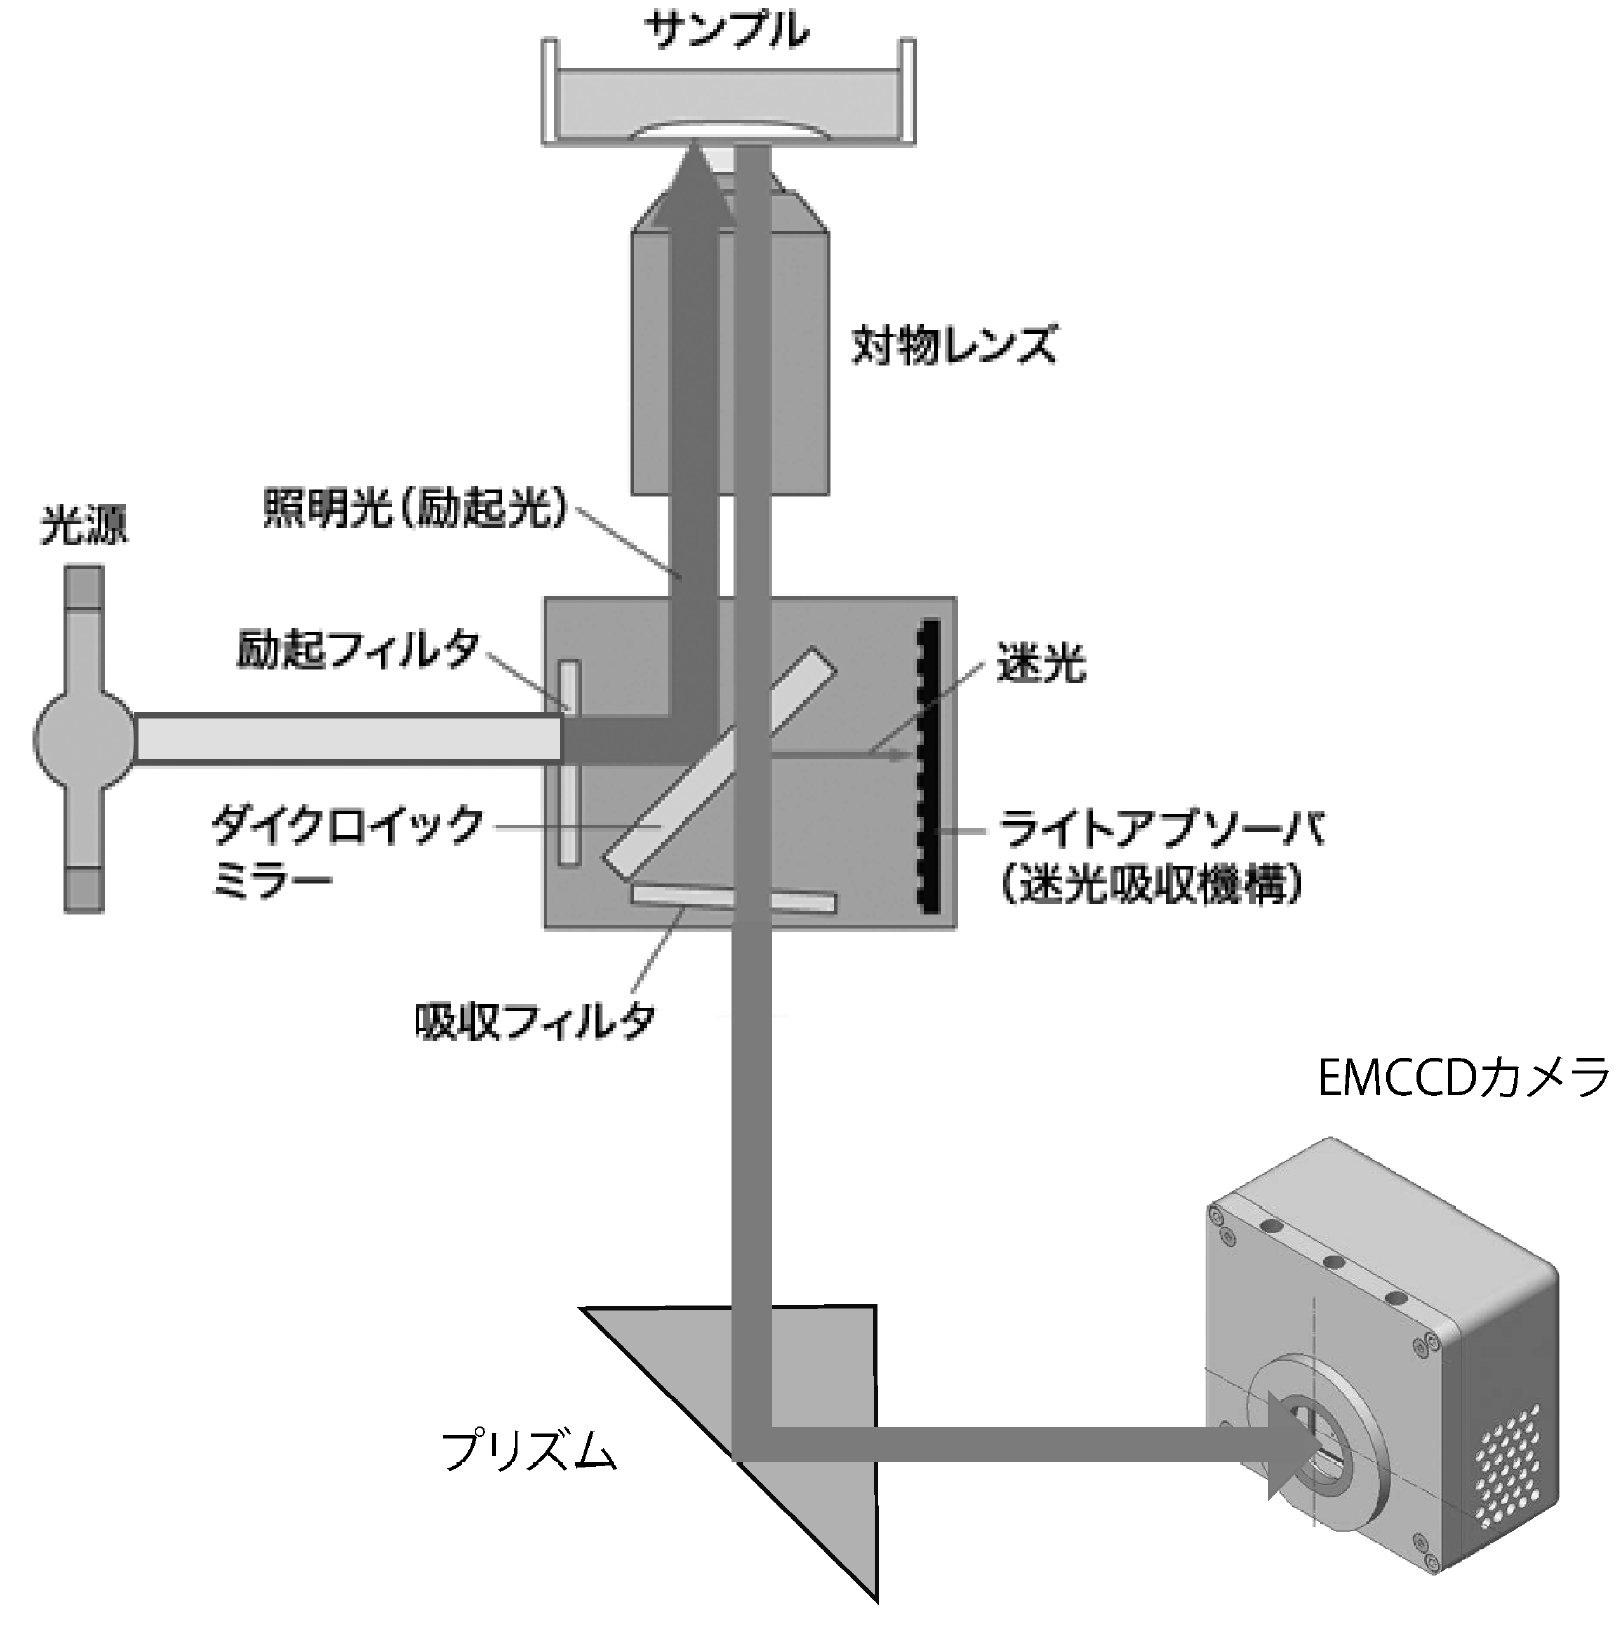
\includegraphics[width=7cm]{scope.png}
    \caption{蛍光顕微鏡の光学配置図.(出典:テキスト\cite{text})}
    \label{fig:scope}
\end{figure}

\subsubsection{フローチャンバーの作製}
実験を始める前に,次の手順でフローチャンバーを作製した.
まず,厚さ\SI{30}{\um}の両面テープを約\SI{3}{\mm}の幅にして2枚切りとり,土台となるカバーガラス(\SI{24}{\mm}$\times$\SI{32}{\mm})の上に\SI{1}{\cm}弱の隙間を空けて貼った.
次に,その上に正方形のカバーガラス(\SI{18}{\mm}$\times$\SI{18}{\mm})を載せた.
このときにできる,二枚のカバーガラスと両面テープに挟まれた領域をチャンバーとして用いた.
最後に,フローチャンバーの流路に沿ってマーカーで線を入れた.
また,土台となるカバーガラスの片隅にも印をつけ,実験では溶液の入れる向きを揃えるようにした.

\subsubsection{アクチン滑り運動の蛍光観察}
まず,カゼイン(\SI{0.2}{\mg\per\milli\liter})\SI{6}{\micro\liter}をピペットで取り出し,チャンバー内に流し込んだ.
次に,モティリティバッファー(\SI{20}{\milli\Molar}\,PIPES\,pH7.2,\SI{5}{\milli\Molar}\,MgSO$_4$,\SI{1}{\milli\Molar}\,EGTA)\SI{4}{\micro\liter}を入れたチューブに,\SI{1}{\mg\per\milli\liter}骨格筋ミオシン\SI{2}{\micro\liter}を入れてよく撹拌し,2分間待った.
その間,モティリティバッファー\SI{15}{\micro\liter}をチャンバーの片側から流し込み,反対側にろ紙を当てて,チャンバー内の溶液を交換した(ガラス面に付着しない余剰のカゼインを洗い流した).
次に,先ほど用意したミオシン溶液にKCl(\SI{0.1}{\Molar},\SI{10}{\micro\liter})を加えてよく撹拌し,約30秒待った後,このうち\SI{6}{\micro\liter}をチャンバーに流し込み,2分間待った.
その後,カゼイン\SI{15}{\micro\liter}をチャンバーに入れ,余剰のミオシンを洗い流した.
次に,蛍光アクチン溶液\SI{6}{\micro\liter}をチャンバーに流し込んだ.
2分間待った後,退色防止剤と脱酸素剤入りのカゼイン溶液\SI{15}{\micro\liter}を流し込み,余剰のアクチンを洗い流した.
こうして用意した試料を蛍光顕微鏡で観察し,ガラス面上でのミオシンとアクチンの結合状態を確認した.

その後,試料にATP濃度\SI{1}{\milli\Molar}の溶液(カゼイン,退色防止剤と脱酸素剤入り)を\SI{6}{\micro\liter}流し込み,蛍光アクチンフィラメントの滑る様子を顕微鏡で撮影した.
同様に,ATP濃度を\SI{200}{\micro\Molar},\SI{50}{\micro\Molar},\SI{10}{\micro\Molar}の溶液についても同様の撮影を行った.

こうして撮影した画像をaviファイルに変換し,画像解析用ソフトウェア(Mark2)上でアクチンの滑り運動の平均速度を求めた.
具体的には,直線的に滑っているアクチンの先端または後端の座標を3~50フレーム単位で5個だけ記録し,それをもとに移動距離と時間について線形近似を行い,フィッティング直線の傾きとして平均移動速度を得た.
また,各ATP濃度について異なる5個のアクチンを選び,それぞれの平均移動速度を求めた.

\subsection{結果と考察}
\subsubsection{水銀ランプと励起フィルターの透過光のスペクトル}

\begin{figure}[htbp]
    \centering
    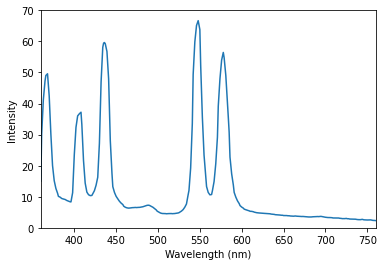
\includegraphics[width=10cm]{Hglamp.png}
    \caption{水銀ランプのスペクトル.波長\SI{368}{\nm}, \SI{408}{\nm}, \SI{436}{\nm}, \SI{548}{\nm}, \SI{578}{\nm}にピークが見られた.}
    \label{fig:Hglamp}
\end{figure}

\begin{table}[htbp]
    \centering
    \caption{水銀ランプのスペクトルのピークにおける波長(測定値)と,水銀の輝線の波長(理論値,値は理科年表\cite{nenpyo}より引用)との比較.}
    \label{tab:Hglamp}
    \begin{tabular}{c|c}
        測定値(\si{\nm}) & 理論値(\si{\nm}) \\
        \hline\hline
        368 & 366.3 \\
        408 & 407.8 \\
        436 & 435.8 \\
        548 & 546.1 \\
        578 & 577.0 \\
        \hline 
    \end{tabular}
\end{table}

まず,水銀ランプのスペクトルには,複数のピークが見られた(図\ref{fig:Hglamp}).
これらの波長を,水銀の輝線の理論値と比較すると,表\ref{tab:Hglamp}のようになった.
これより,測定値は理論値から最大で\SI{2}{\nm}程度ずれることが分かった.
また,測定値は理論値よりも大きい傾向にあることも分かった.
ただし,水銀ランプや測定器の詳細が分からなかったので,これらについて考察はできなかった.

\begin{figure}[htbp]
    \centering
    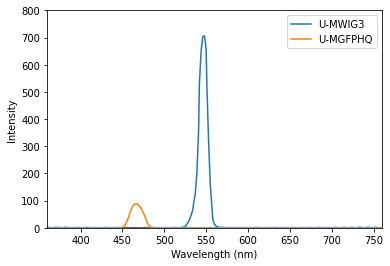
\includegraphics[width=10cm]{filters.png}
    \caption{励起フィルターの透過光のスペクトル.U-MWIG3を用いた場合には波長\SI{548}{\nm}にピークが見られ,U-MGFPHQを用いた場合には波長\SI{466}{\nm}にピークが見られた.}
    \label{fig:filter}
\end{figure}

\begin{figure}[htbp]
    \centering
    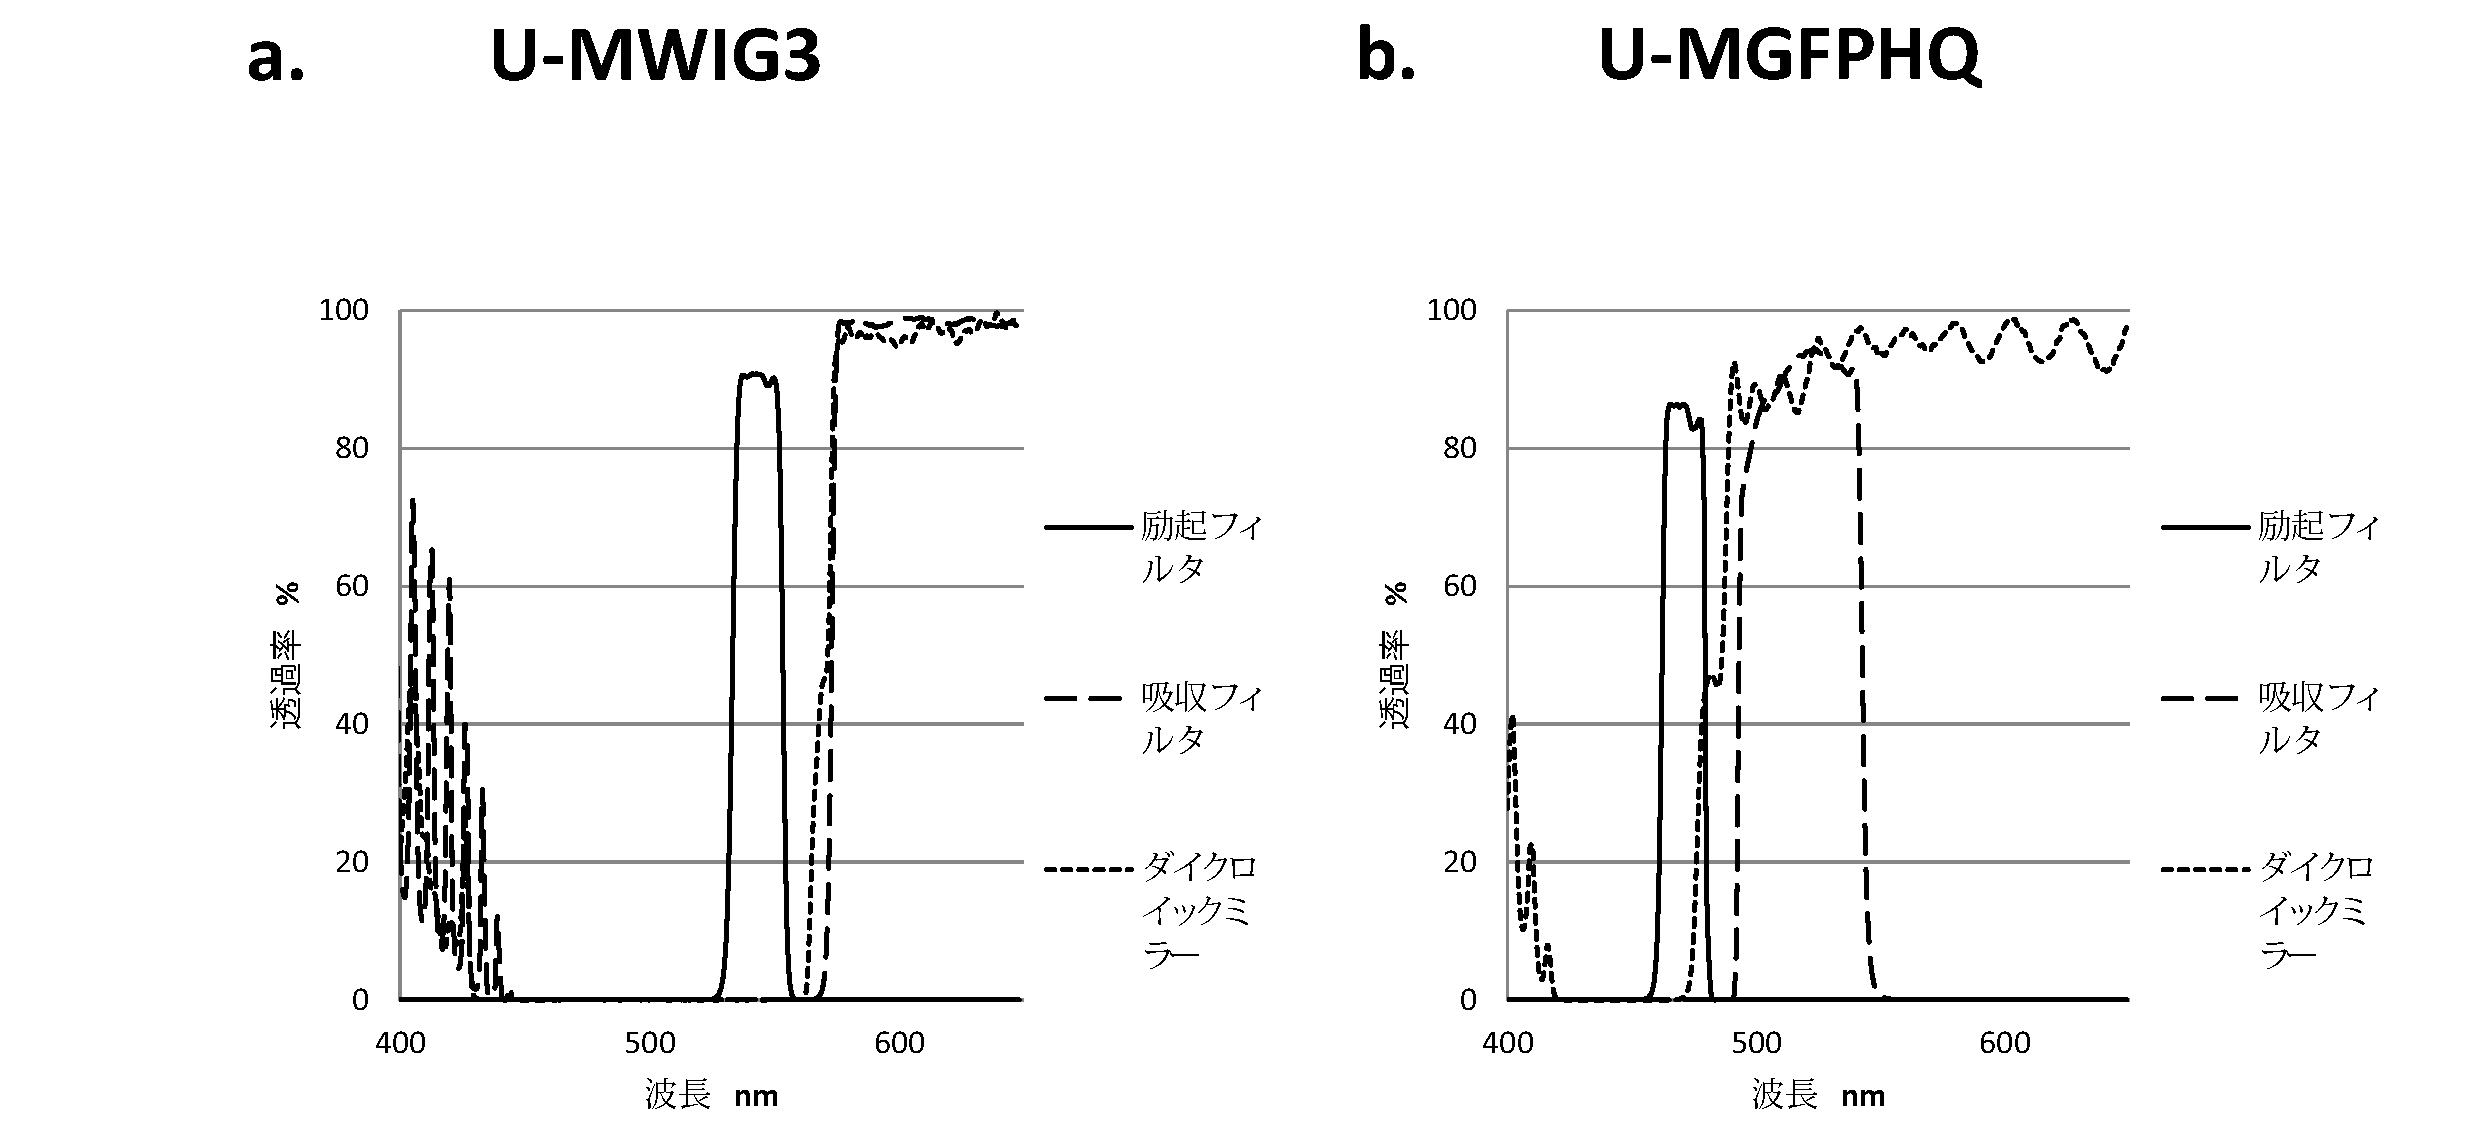
\includegraphics[width=14cm]{filters_text.png}
    \caption{蛍光ミラーユニットの分光特性.(a)はU-MWIG3であり,(b)はU-MGFPHQ.(出典:テキスト\cite{text})}
    \label{fig:filter_text}
\end{figure}

一方で,励起フィルターの透過光のスペクトルは,どちらの蛍光ミラーユニットに対してもただ一つだけピークが見られた(図\ref{fig:filter}).
そのピークの波長は,U-MWIG3の場合\SI{548}{\nm},U-MGFPHQの場合\SI{466}{\nm}であった.
これは,蛍光ミラーユニットの分光特性(図\ref{fig:filter_text})に示した励起フィルターの透過率が約80\%~90\%に達する波長領域と合致する.
また,U-MGFPHQを用いた場合と比べてU-MWIG3を用いた場合の方がピークの強度が数倍大きかった.
これは,後者の場合に水銀ランプのピーク波長(\SI{548}{\nm})の光を透過したためと考える.

\subsubsection{ミオシンとアクチンの相互作用の分子メカニズム}

\begin{figure}[htbp]
    \centering
    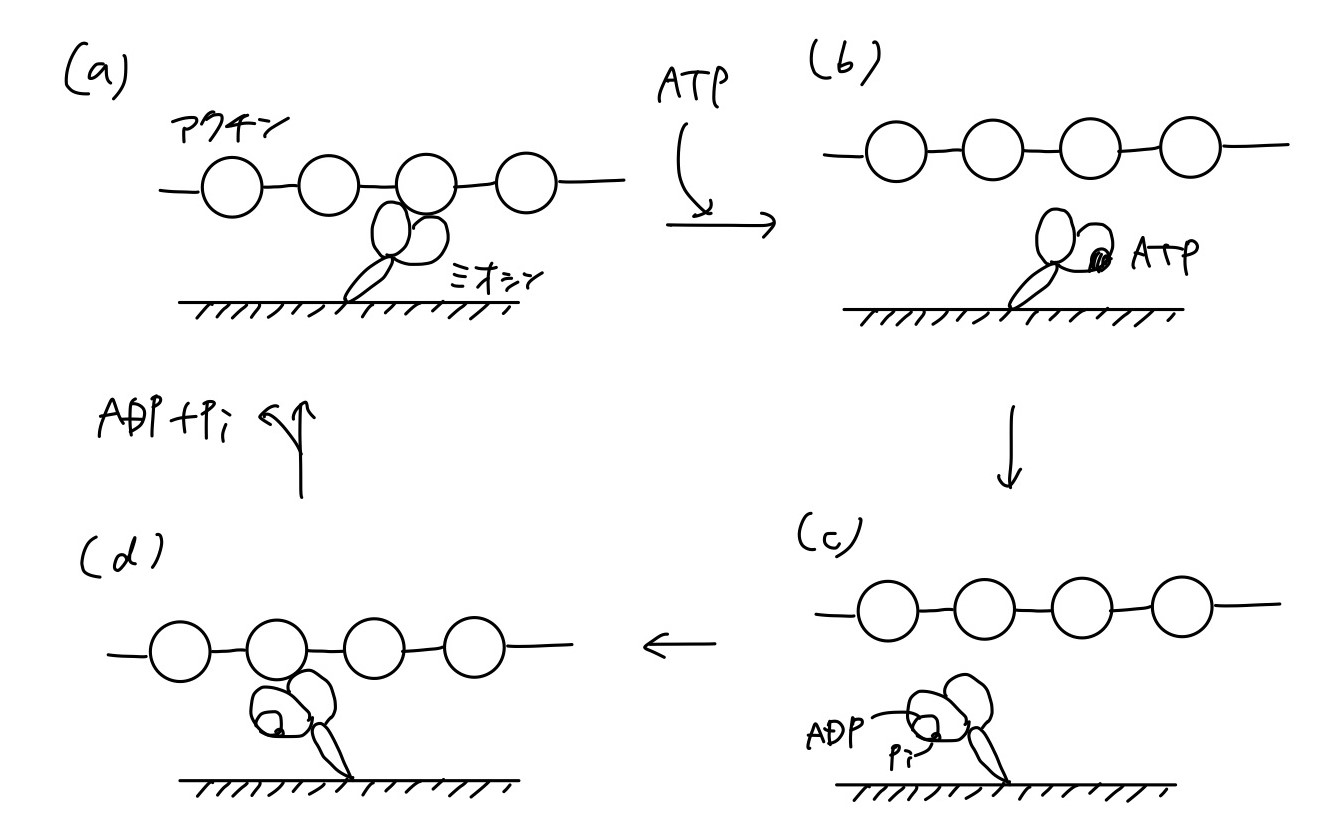
\includegraphics[width=10cm]{actin_myosin.jpg}
    \caption{アクチンとミオシンの相互作用.(a)ATPの結合していないミオシンはアクチンと強く結合する.(b)ATPの結合したミオシンはアクチンから素早く離れる.(c)ATPの加水分解に伴いミオシンが構造変化する(リカバリーストローク).(d)ADPと無機リン酸の結合したミオシンは再びアクチンと結合する.その後,ADPと無機リン酸が遊離して構造変化し,アクチンを押し出す(パワーストローク).}
    \label{fig:actin_myosin}
\end{figure}

ここでは,Lymn \& Taylor(1971)の研究(参考文献\cite{actin_myosin})を参考に,ATP\,1分子の加水分解に伴うミオシンとアクチンの相互作用について述べる.
最初に,反応の概略を説明する.
まず,ATPが結合していない状況では,ミオシンフィラメントから突き出たミオシンヘッドはアクチンフィラメントと強く結合している(図\ref{fig:actin_myosin}(a)).
ミオシンヘッドにATP分子が結合すると,アクチンフィラメントとの結合が切れる(図\ref{fig:actin_myosin}(b)).
そして,結合したATP分子の加水分解に伴ってミオシンは構造変化する(図\ref{fig:actin_myosin}(c)).
この過程はリカバリーストロークと呼ばれる.
このとき,加水分解してできたADPと無機リン酸はミオシンヘッドに結合したままである.
次に,このミオシンヘッドがアクチンフィラメントと再び結合する(図\ref{fig:actin_myosin}(d)).
その後,ミオシンヘッドはADPと無機リン酸を放出し,アクチンフィラメントに結合したまま構造変化する.
この過程はパワーストロークと呼ばれ,このときアクチンフィラメントはミオシンヘッドと同じ向きに動く\footnote{実際には,無機リン酸が遊離してからパワーストロークが起こり,最後にADPが遊離する\cite{life_science}.しかし,ここでは単純にこれらが同時に起こるものと考える.}.
こうして最初の状態に戻り,このサイクルが繰り返される.

次に,以上の機構に基づき,アクチンの滑り速度$v$とATP濃度との関係を考察する.
図\ref{fig:actin_myosin}をもとに化学反応式を書くと次のようになる(ただし,\ce{A}はアクチン,\ce{M}はミオシンを意味する.):
\begin{equation}
    \ce{AM + ATP ->[${k_1}$] M-ADP-P + A <=>[${k_2}$][${k_{-2}}$] AM-ADP-P ->[${k_3}$] AM + ADP + P} 
\end{equation}
ここでは,(a)から(c)へは速やかに変化すると仮定し,(d)から(c)への逆反応を新たに考慮した.
また,(a)から(c)への反応の速度定数を$k_1$,(c)から(d)への反応の速度定数を$k_2$,その逆反応の速度定数を$k_{-2}$,(d)から(a)への反応の速度定数を$k_3$とした.
この最後の反応において,アクチンフィラメントが動く.
そこで,この一連の化学反応をもとに,各物質の濃度変化を記述する式を立てると,
\begin{align}
    \dv{[\ce{M-ADP-P}]}{t} &= k_1[\ce{AM}][\ce{ATP}] - k_2[\ce{M-ADP-P}][\ce{A}] \label{ac}\\
    \dv{[\ce{AM-ADP-P}]}{t} &= k_2[\ce{M-ADP-P}][\ce{A}] -(k_{-2} + k_3)[\ce{AM-ADP-P}] \label{cd} \\
    \dv{[\ce{ADP}]}{t} &= k_3[\ce{AM-ADP-P}] =: v_{\mathrm{r}} \label{da}
\end{align}
となる.
ここで,反応の中間体である\ce{M-ADP-P}および\ce{AM-ADP-P}は速やかに平衡に到達すると仮定すると,式\eqref{ac}および式\eqref{cd}はゼロとみなせる(断熱近似).
このことから,
\begin{equation}
    [\ce{AM}] = \frac{(k_{-2} + k_3)[\ce{AM-ADP-P}]}{k_1[\ce{ATP}]} \label{amadpp}
\end{equation}
と書ける.
次に,この反応を通してミオシン分子の数は一定なので,
\begin{equation}
    [\ce{AM}] + [\ce{M-ADP-P}] + [\ce{AM-ADP-P}]
\end{equation}
は一定である.
また,中間体は平衡にあるので,$[\ce{M-ADP-P}]$および$[\ce{AM-ADP-P}]$は一定である.
よって,次のパラメータ$M$は一定である:
\begin{equation}
    M := [\ce{AM}] + [\ce{AM-ADP-P}]
\end{equation}
よって,式\eqref{amadpp}より
\begin{align}
    &M = \qty(1 + \frac{k_{-2} + k_3}{k_1[\ce{ATP}]})[\ce{AM-ADP-P}]  \\
    &[\ce{AM-ADP-P}] = \frac{k_1 M[\ce{ATP}]}{[\ce{ATP}] + \frac{k_1}{k_{-2} + k_3}}
\end{align}
となる.
これと式\eqref{da}から,ミオシンがADPと無機リン酸を放出する過程の反応速度は,
\begin{equation}
    v_{\mathrm{r}} = \frac{V_{\mathrm{r,max}}[\ce{ATP}]}{[\ce{ATP}] + K_m}
\end{equation}
と求まる.
ただし,
\begin{align}
    V_{\mathrm{r,max}} &= k_1 k_3 M\\
    K_m &= \frac{k_1}{k_{-2} + k_3}  
\end{align}
とした.
ここで,この反応1回あたりにアクチンフィラメントが進む距離を$d$とおくと,アクチンフィラメントの滑り速度は
\begin{equation}
    v = dv_{\mathrm{r}} = \frac{V_{\mathrm{max}}[\ce{ATP}]}{[\ce{ATP}] + K_m} \label{micmen}
\end{equation}
と書ける.
ただし,
\begin{equation}
    V_{\mathrm{max}} = dV_{\mathrm{r,max}} = dk_1 k_3 M
\end{equation}
とした.
これより,ATP濃度とアクチンの滑り速度の関係はMichaelis-Mentenの公式によって記述できると考える.

\subsubsection{アクチンの滑り速度とATP濃度の関係}

\begin{table}[htbp]
    \centering
    \caption{各ATP濃度におけるアクチンの平均滑り速度.滑り速度は直線的に動く十分長いアクチンフィラメントを,ATP濃度ごとに5つずつ選んで測定した.平均滑り速度はその平均値である.平均滑り速度の誤差は,この5つの測定値の不偏標準偏差をサンプル数5の平方根で割った値にとった.}
    \label{tab:velocity}
    \begin{tabular}{c|c}
        ATP濃度(\si{\micro\Molar}) & 平均滑り速度(\si{\nm\per\second}) \\
        \hline\hline
        10 & 66$\pm$7 \\
        50 & 850$\pm$50 \\
        200 & 2100$\pm$130 \\
        1000 & 3100$\pm$300 \\
        \hline
    \end{tabular}
\end{table}

\begin{figure}[htbp]
    \centering
    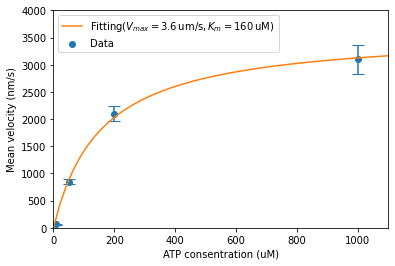
\includegraphics[width=10cm]{mmfit.png}
    \caption{アクチンの滑り速度とATP濃度の関係.Michaelis-Mentenの公式を用いたフィッティングの結果も示す.}
    \label{fig:mmfit}
\end{figure}

実験の結果,各ATP濃度におけるアクチンの平均滑り速度は表\ref{tab:velocity}のようになった.
これより,ATP濃度が高いほど平均滑り速度は大きくなることが分かる.
ここで,ATP濃度$[\ce{ATP}]$と平均滑り速度$v$の間にはMichaelis-Mentenの式\eqref{micmen}が成り立つと考え,フィッティングを行って最大速度$V_{\mathrm{max}}$およびMichaelis-Menten定数$K_m$を計算した.
ただし,ここで平均滑り速度の誤差を考慮するとこれらのパラメータの誤差が非常に大きくなってしまったので,誤差を考慮せずにフィッティングを行った.
その結果,
\begin{align}
    V_{\mathrm{max}} &= \SI[separate-uncertainty]{3.6 \pm 0.2}{\um\per\second} \\
    K_m &= \SI[separate-uncertainty]{160 \pm 30}{\micro\Molar}
\end{align}
と求まった.
図\ref{fig:mmfit}より,フィッティングは実験データをよく説明している.

\subsubsection{細胞におけるミオシンの役割}

\begin{figure}[htbp]
    \centering
    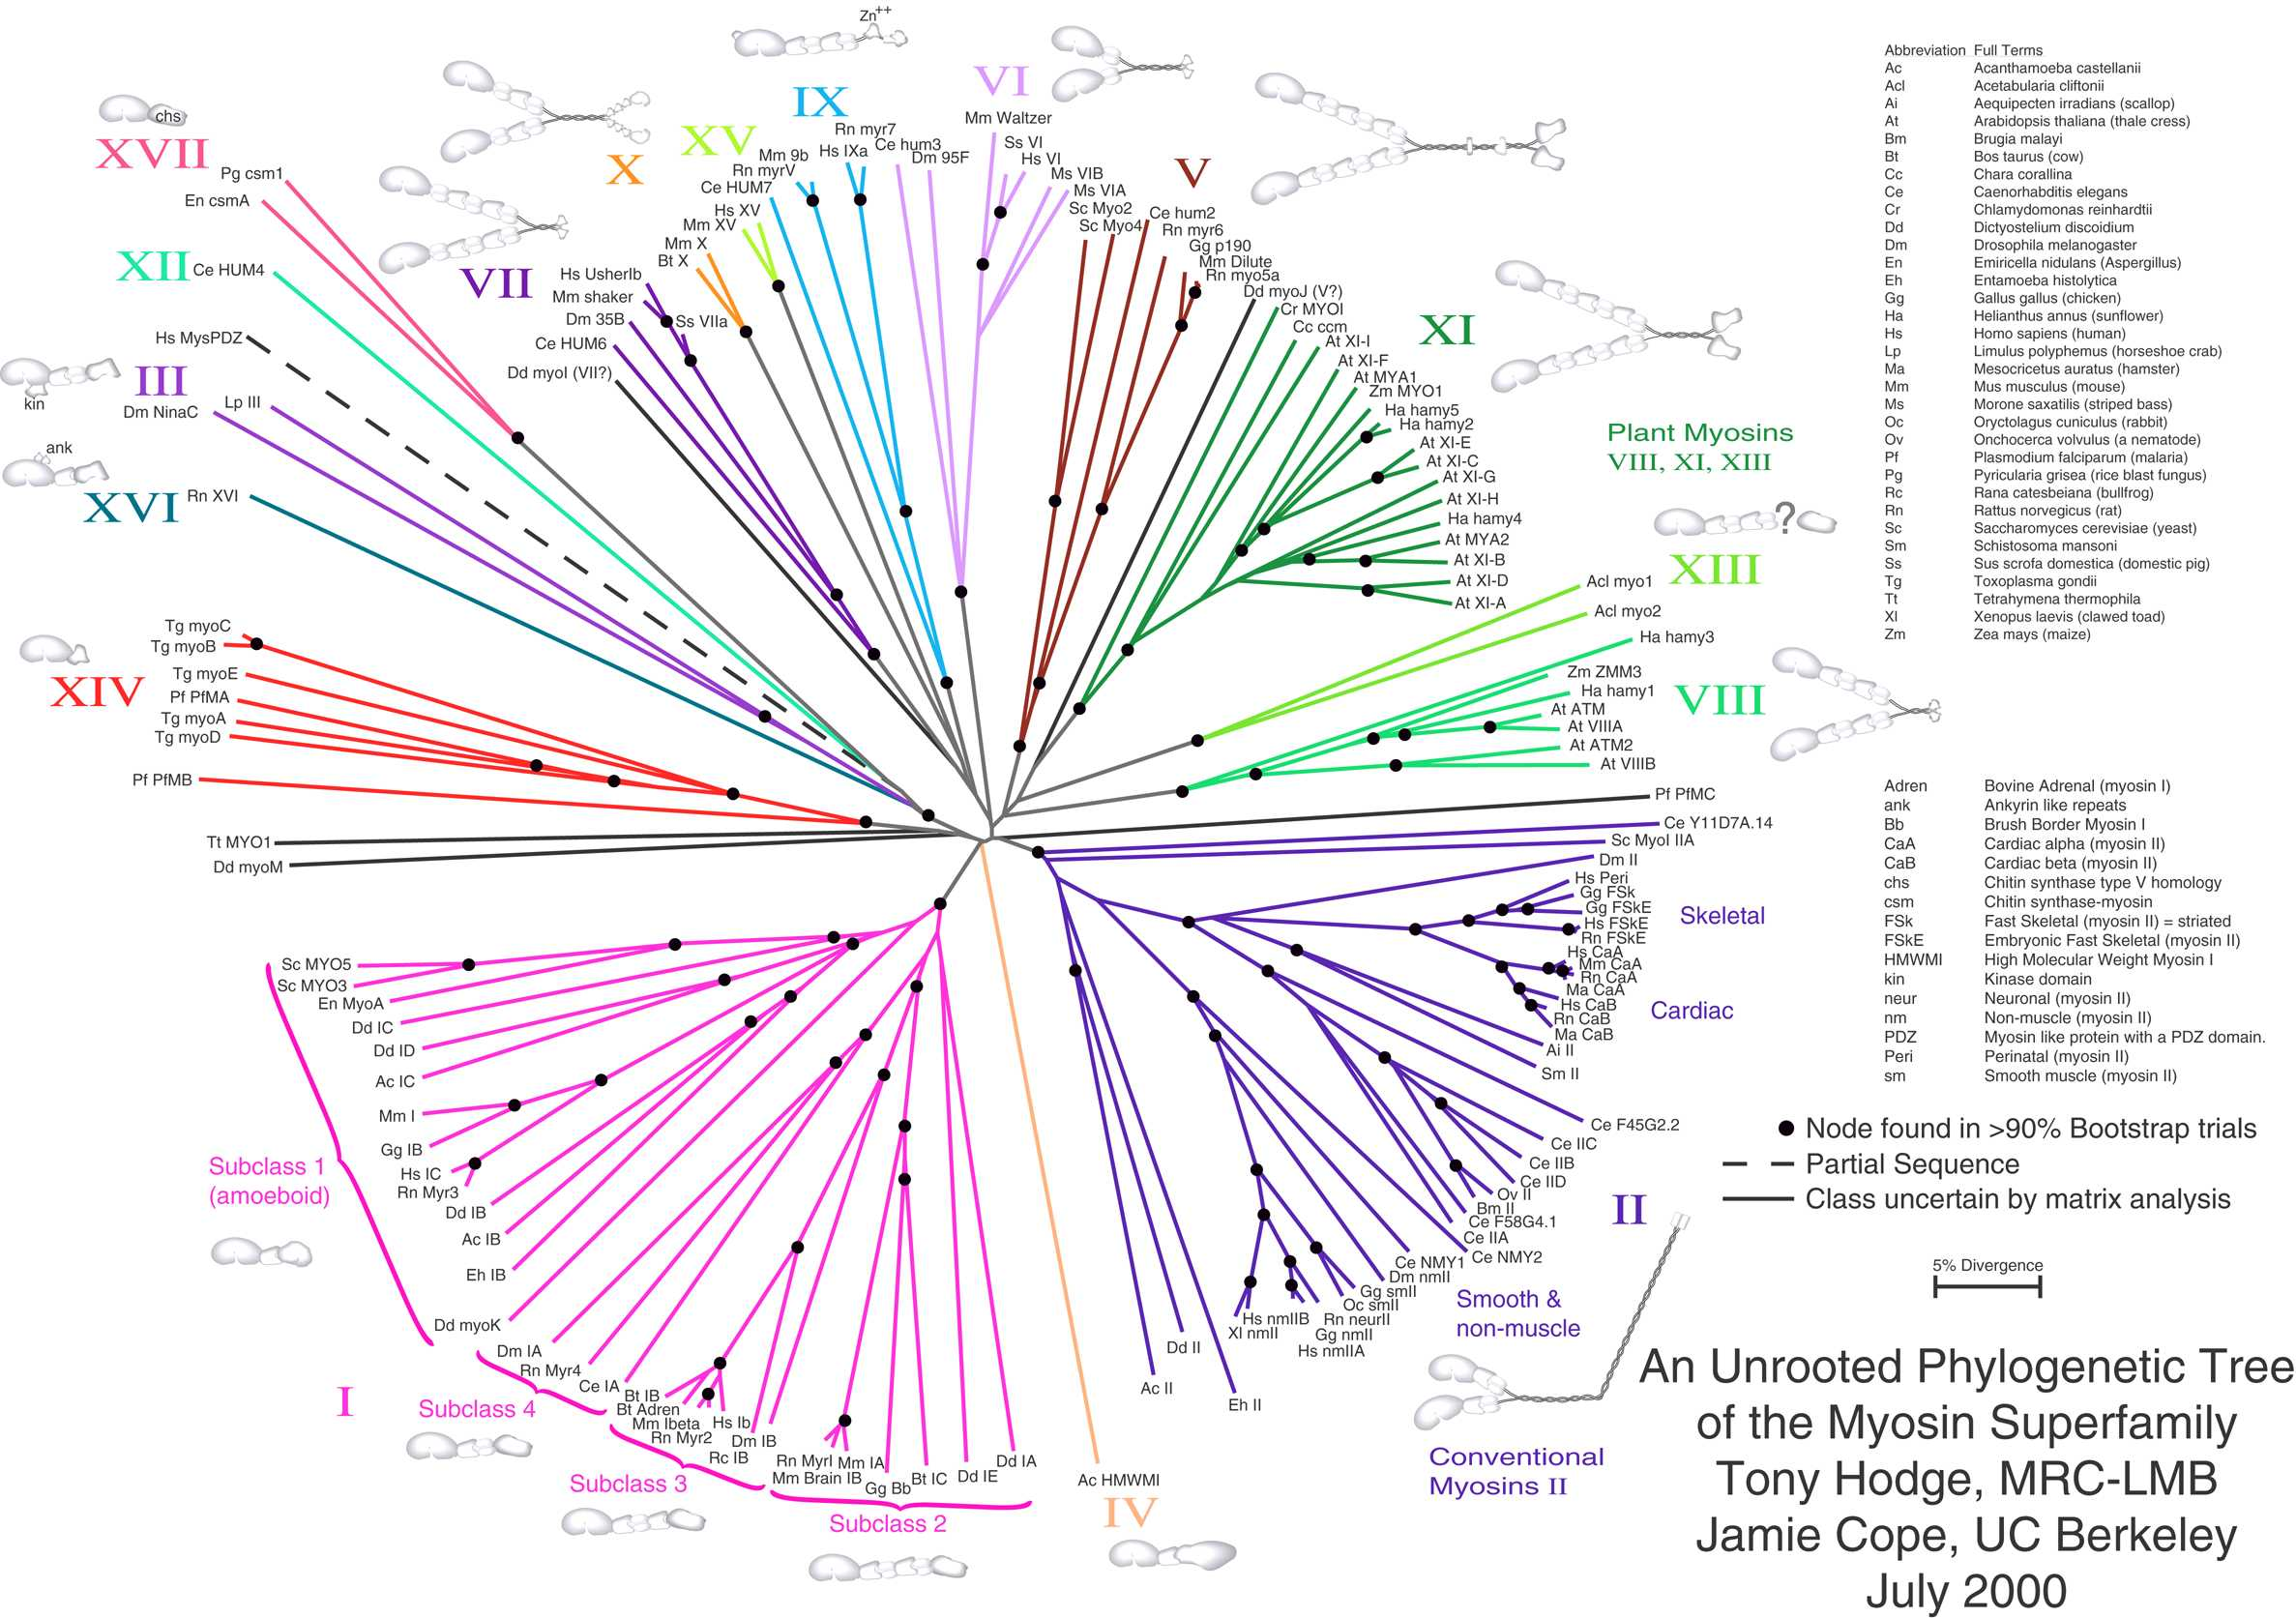
\includegraphics[width=13cm]{MyosinUnrootedTree.jpg}
    \caption{ミオシンの系統樹(出典:Hodge \& Cope(2000)\cite{myosin_tree})}
    \label{fig:myosin_tree}
\end{figure}

ミオシンはモータードメイン(頭部のうち,アクチンやATPと相互作用する部分)の塩基配列に基づく系統関係にしたがってローマ数字で分類されており,その種類はミオシン\ajRoman{1}からミオシンXVIIまで多岐にわたる(図\ref{fig:myosin_tree}).
ここでは,真核生物の中では比較的よく見られる\cite{myosin_paper}ミオシン\ajRoman{1},ミオシン\ajRoman{2},ミオシン\ajRoman{5}について紹介する.
この部分の説明は,Sellers(1999)\cite{myosin_paper},MBInfoの記事\cite{what_is_myosin},Mclntosh \& Ostap(2016)\cite{myosin_1},生命科学のテキスト\cite{life_science}をもとに書いた.

ミオシン\ajRoman{1}は単量体で存在する.
また他のミオシンとは異なる尾部を持ち,これにより複数のアクチンフィラメントや脂質膜に結合できる.
その機能としては,細胞膜の張力の生成およびその制御,細胞膜の形成,アクチン構造の変化,細胞内輸送などが挙げられる.

一方,ミオシン\ajRoman{2}は基本的には二量体として存在し,すべての真核生物に共通して存在する.
その特徴として,尾部同士が相互作用して多数結合し,両極性の太いフィラメントを形成することが挙げられる.
このミオシンフィラメントは外向きにミオシンの頭部が飛び出しており,それがアクチンフィラメントと相互作用することで,アクチンフィラメントとの間で滑り運動が起こる.
これは,今回の実験で観察した現象である.
生体内では,とくに筋細胞内のサルコメアで見られ,筋収縮の働きを担う.
ほかにも,細胞内でアクチンによる細胞骨格ネットワークと相互作用し,細胞シグナル伝達,細胞の運動,細胞分裂,細胞運命の決定などの過程に寄与する.

ミオシン\ajRoman{5}も二量体として存在するが,ミオシン\ajRoman{2}よりも頸部が長い.
また,フィラメントを形成するわけではなく単体で働く.
ミオシン\ajRoman{5}は尾部に輸送小胞を結合させ,頭部がアクチン繊維と相互作用することで,アクチン繊維状を「歩く」ように小胞を運搬する.
このような能動輸送により,受動輸送(拡散)よりも素早く物質を運ぶことができる.

このように,一言にミオシンといっても,その構造や働き方は様々である.

\begin{thebibliography}{99}
    \bibitem{text}
        「物理学実験\ajRoman{2}」解説書「生物物理学」2021年度 東京大学理学部物理学科
    \bibitem{chemsta}
        Chem-Station,2008年ノーベル化学賞『緑色蛍光タンパク質の発見と応用』\\
        \url{https://www.chem-station.com/blog/2009/01/2008.html}
    \bibitem{kahaku}
        国立科学博物館,蛍光タンパク質が教えてくれるもの
        \url{https://www.kahaku.go.jp/userguide/hotnews/theme.php?id=0001286268353983&p=4}
    \bibitem{refolding}
        Enoki, S., Saeki, K., Maki, K., \& Kuwajima, K. (2004). Acid denaturationand and refolding of green fluorescent protein. \textit{Biochemistry}, 43(44), 14238-14248.
    \bibitem{nenpyo}
        国立天文台編「理科年表2019」丸善出版
    \bibitem{actin_myosin}
        Lymn, R.W., Taylor, E.W. (1971). Mechanism of adenosine triphosphate hydrolysis by actomyosin. \textit{Biochemistry}, 10(25), 4617–4624.
    \bibitem{myosin_tree}
        Hodge, T. \& Cope, M.J.T.V. (2000). A Myosin Family Tree. \textit{Journal of Cell Science}, 113, 3353-3354.
    \bibitem{myosin_paper}
        Sellers, J. R. (1999). Myosins: a diverse superfamily. \textit{Biochim Biophys Acta.}, 1496(1), 3-22.
    \bibitem{what_is_myosin}
        MBInfo, What is Myosin? 
        \url{https://www.mechanobio.info/cytoskeleton-dynamics/what-are-motor-proteins/what-is-myosin/}
    \bibitem{myosin_1}
        Mclntosh, B. B. \& Ostap, E. M. (2016). Myosin-I molecular motors at a glance. \textit{Journal of Cell Science}, 129(14), 2689-2695. 
    \bibitem{life_science}
        東京大学生命科学教科書編集委員会「理系総合のための生命科学 第4版」羊土社


\end{thebibliography}
\end{document}